\section{Analysis} \label{sec:Charmonia_Analysis}

In this section, two related analyses of the charmonium production in \Runpp and \RunPbPb collisions at $\sqrtsnn = \SI{5.02}{\TeV}$, are described. The measurements are performed in the \mumu decay channel using data recorded with the CMS detector. In both of the analyses, I made significant contributions in the signal extraction, acceptance studies and determination of the systematic uncertainties related to the fitting procedure.

The first analysis~\cite{CMS_JPsi_PbPb_5p02TeV} studies the modification of the prompt and nonprompt \JPsi meson production in \RunPbPb compared to \Runpp collisions at the same energy. To accomplish this, the nuclear modification factor of \JPsi mesons is measured in different collision centrality bins, and \JPsi-meson \pt and rapidity (\rap) ranges. The second analysis~\cite{CMS_Psi2S_PbPb_5p02TeV} probes the nuclear modification of \PsiP mesons relative to \JPsi mesons, by measuring the double ratio of \PsiP over \JPsi yields in \RunPbPb relative to \Runpp collisions, defined as:

\begin{equation}
 \rho^{\PsiP/\JPsi} = \frac{\left(N_{\PsiP}/N_{\JPsi}\right)_{\PbPb}}{\left(N_{\PsiP}/N_{\JPsi}\right)_{\pp}}
\end{equation}

One advantage of measuring the double ratio of charmonium yields is that the acceptance and efficiency of the two charmonium states cancel in the ratio due their similar masses and production mechanisms. For this reason, as well as the limited statistics of the \PsiP mesons compared to \JPsi mesons, the second analysis was published first and relatively fast after the data was taken, while the first analysis was more elaborate and required more time to complete.


The \Runpp and \RunPbPb datasets employed are introduced in \sect{sec:Charmonia_Analysis_Data}, while the charmonium simulations are listed in \sect{sec:Charmonia_Analysis_MC} and the event selection is presented in \sect{sec:Charmonia_Analysis_Selection}. The procedure used to extract the prompt and nonprompt \JPsi-meson yields is explained in \sect{sec:Charmonia_Analysis_JPsiYieldExtraction} and the extraction of the single ratios of \PsiP over \JPsi meson yields is detailed in \sect{sec:Charmonia_Analysis_PsiPoverJPsiRatioExtraction}. The charmonium efficiency and acceptance are derived in \sect{sec:Charmonia_Analysis_Efficiency}. \sect{sec:Charmonia_Analysis_JPsiYieldSystematics} and \sect{sec:Charmonia_Analysis_PsiPoverJPsiRatioSystematics} report the systematic uncertainties associated to the measurement of the \JPsi-meson yields and the double ratio of charmonium yields, respectively.


\subsection{Dataset} \label{sec:Charmonia_Analysis_Data}

The measurement of the nuclear modification of \PsiP and \JPsi mesons is performed using data recorded in 2015 by the CMS detector, in \Runpp and \RunPbPb collisions at $\sqrtsnn = \SI{5.02}{\TeV}$. The main datasets employed in the analyses, called \textit{DoubleMu0} for \Runpp and \textit{HIOniaDoubleMu0} for \RunPbPb, consist of events selected by the CMS trigger system, requiring the presence of at least two L1 muon candidates. An additional dataset selecting also L1 double muon events, referred as \textit{HIOniaPeripheral30100}, is employed to measure the charmonium production in peripheral \RunPbPb collisions (centrality range $30-100\%$), since it accumulated more integrated luminosity than HIOniaDoubleMu0\footnote{The data rate of HIOniaDoubleMu0 was reduced during part of the \RunPbPb run because it exceeded the bandwidth threshold of the Tier-0 computing centre.}.

The \Runpp and \RunPbPb datasets were reconstructed with CMSSW 7.5.8, making use of the standard \Runpp and heavy-ion specific reconstruction algorithms employed during the data-taking period, respectively. After a meticulous check of the quality of the data by the CMS collaboration, the content of the datasets were filtered excluding events in which the tracker or the muon system were not operating in proper conditions. The total integrated luminosity of the data samples is presented in \tab{tab:lumi}.

\begin{table}[htb!]
 \centering
 \begin{tabular}{c c c}
  System & Primary dataset & Integrated luminosity \\
  \hline
  \RunPbPb & HIOniaDoubleMu0 & 351~\mubinv \\
  \RunPbPb & HIOniaPeripheral30100 & 464~\mubinv \\
  \Runpp & DoubleMu0 & 28~\pbinv \\
 \end{tabular}
 \caption{Total integrated luminosity of each dataset used in the analysis of the charmonium nuclear modification in \Runpp and \RunPbPb collisions at $\sqrtsnn = \SI{5.02}{\TeV}$.}
 \label{tab:lumi}
\end{table}

%%------------------------------------------------------------%%
\subsection{Charmonium simulations} \label{sec:Charmonia_Analysis_MC}

The production of \PsiP and \JPsi mesons is described using fully reconstructed Monte-Carlo simulated samples. The simulations were made separately for charmonia produced directly from the hard scattering (prompt \JPsi and \PsiP mesons), and for \JPsi mesons produced from the decay of b hadrons (nonprompt \JPsi mesons), for both \Runpp and \RunPbPb collisions. The prompt \PsiP and \JPsi events were generated with \PYTHIA 8.209~\cite{PYTHIA8}, which models the charmonium production using NRQCD. Regarding the nonprompt \JPsi sample, the b hadrons ($\B^{\pm}, \B^{0}, \overline{\B}^{0}, \B^{0}_{\cPqs}, \overline{\B}^{0}_{\cPqs}$ mesons) were decayed with the \EVTGEN v1.3~\cite{EVTGEN} package interfaced to \PYTHIA 8.209. The CUETP8M1 underlying event \PYTHIA tune~\cite{PYTHIA_TUNE,UE_pp} was used in all samples. 

Moreover, the underlying environment present in \RunPbPb collisions was first simulated with \HYDJET 1.9~\cite{HYDJET} and then embedded to each \PYTHIA signal event, by matching the position of the simulated interaction vertex. The full CMS detector response was simulated in all charmonium simulations, based on \GEANTfour~\cite{GEANT4}, and the \Runpp and \RunPbPb simulated collision events were reconstructed with the corresponding reconstruction algorithms used during 2015 data taking.

In addition, the \RunPbPb simulations were produced in several ranges of charmonium or \B-meson \pt, in order to have similar statistics available in each \pt range. As a result, $w_{\pt}$ weights are used for each meson \pt range to combine the different \RunPbPb simulations and form a continuous \pt spectrum.

Finally, in order to match the centrality distribution of the signal simulations to what is observed in data, each \RunPbPb event is weighed by the average \ncoll corresponding to the centrality range of the simulated collision. The differences between the data and simulated centrality distributions are due to the fact that the signal events were embedded into minimum bias \HYDJET events equally distributed in centrality, while the production of charmonium in data is biased towards more central collisions (i.e. scales with \ncoll). Thus, in summary, each \RunPbPb charmonium simulated event is weighed by:

\begin{equation}
 w_{\MC} = N^{gen} \frac{w_{p_{T}} \cdot \ncoll}{\sum_{i=1}^{N^{gen}}\left(w_{p_{T}}^{i} \cdot \ncoll^{i}\right)}
\end{equation}

where the weights are normalised so that their sum is effectively equal to the number of generated events. The list of charmonium simulations are summarized in \tab{tab:CharmoniaMCSamples}.

\begin{table} [hbt!]
  \centering
  \resizebox{\textwidth}{!}{
    \renewcommand{\arraystretch}{1.5}
    \begin{tabular}{c c c c c}
      \hline
      Process & Generator & Criteria & Acceptance & Events \\
      \hline
      \multirow{7}{*}{$\PbPb \to \JPsiToMuMu$} & \multirow{7}{*}{\PYTHIA+\HYDJET} & $\JPsi \pt [ 0,   3]~\GeVc$ & $2.5{\times}10^{-1}$ & 150659  \\
       & & $\JPsi\, \pt [ 3,   6]~\GeVc$ & $1.7{\times}10^{-1}$ & 3842575 \\
       & & $\JPsi\, \pt [ 6,   9]~\GeVc$ & $2.0{\times}10^{-2}$ & 2268977 \\
       & & $\JPsi\, \pt [ 9,  12]~\GeVc$ & $4.0{\times}10^{-3}$ & 168628  \\
       & & $\JPsi\, \pt [12,  15]~\GeVc$ & $1.2{\times}10^{-3}$ & 155793  \\
       & & $\JPsi\, \pt [15,  30]~\GeVc$ & $7.2{\times}10^{-4}$ & 104729  \\
       & & $\JPsi\, \pt [30,\inf]~\GeVc$ & $3.3{\times}10^{-5}$ & 47059   \\
      \hline
      \multirow{6}{*}{$\PbPb \to \PsiPToMuMu$} & \multirow{6}{*}{\PYTHIA+\HYDJET} & $\PsiP \pt [ 0,   3]~\GeVc$ & $2.4{\times}10^{-1}$ & 96623   \\
       & & $\PsiP\, \pt [ 3,   6]~\GeVc$ & $2.1{\times}10^{-1}$ & 89880   \\
       & & $\PsiP\, \pt [ 6,   9]~\GeVc$ & $3.1{\times}10^{-2}$ & 98836   \\
       & & $\PsiP\, \pt [ 9,  12]~\GeVc$ & $6.4{\times}10^{-3}$ & 102038  \\
       & & $\PsiP\, \pt [12,  15]~\GeVc$ & $2.0{\times}10^{-3}$ & 94370   \\
       & & $\PsiP\, \pt [15,\inf]~\GeVc$ & $1.2{\times}10^{-3}$ & 49857   \\
      \hline
      \multirow{7}{*}{$\PbPb \to \BToJPsiToMuMu$} & \multirow{7}{*}{\EVTGEN+\PYTHIA+\HYDJET} & $\B \pt [ 0,   3]~\GeVc$ & $2.7{\times}10^{-1}$ & 140257  \\
       & & $\B\, \pt [ 3,   6]~\GeVc$ & $1.5{\times}10^{-1}$ & 5192754 \\
       & & $\B\, \pt [ 6,   9]~\GeVc$ & $5.0{\times}10^{-2}$ & 1786414 \\
       & & $\B\, \pt [ 9,  12]~\GeVc$ & $1.0{\times}10^{-3}$ & 165143  \\
       & & $\B\, \pt [12,  15]~\GeVc$ & $3.6{\times}10^{-3}$ & 141064  \\
       & & $\B\, \pt [15,  30]~\GeVc$ & $2.1{\times}10^{-3}$ & 107742  \\
       & & $\B\, \pt [30,\inf]~\GeVc$ & $1.4{\times}10^{-4}$ & 41803   \\
      \hline
      $\pp \to \JPsiToMuMu$    & \PYTHIA & & 1.0 & 60830490 \\
      \hline
      $\pp \to \PsiPToMuMu$    & \PYTHIA & & 1.0 & 60830490 \\
      \hline
      $\pp \to \BToJPsiToMuMu$ & \PYTHIA & & 1.0 & 69652510 \\
      \hline
    \end{tabular}
  }
  \caption{Simulations used in the analysis of the charmonium production in \RunPbPb and \Runpp collisions at \SI{5.02}{\TeV}.}
  \label{tab:CharmoniaMCSamples}
\end{table}


% END OF SUBSECTION


\subsection{Event selection} \label{sec:Charmonia_Analysis_Selection}

The charmonium candidates are reconstructed in the dimuon decay channel (i.e. \JPsiToMuMu and \PsiPToMuMu), by pairing opposite-charge muons. Since the \JPsi and \PsiP masses are small ($\text{m}_{\JPsi} = 3.097~\GeVcc$ and $\text{m}_{\PsiP} = 3.686~\GeVcc$), the signal events are dominated by the presence of low \pt muons ($\langle\pt^{\PGm}\rangle \sim 1.6~\GeVc$), contrary to the \PW-boson analysis reported in \chp{sec:WBoson}. The selection used to identify the charmonium events is detailed in this section.

%%------------------------------------------------------------%%
\subsubsection{Minimum bias event selection} \label{sec:Charmonia_Analysis_Selection_EventFilter}

The \Runpp and \RunPbPb minimum bias events are selected by applying a global event filter (GEF) offline to suppress the background events not originating from the inelastic hadronic scattering. The GEF for \Runpp collision events consists of the following filters:
\begin{itemize}
\item Beam-Scraping filter: Requires at least 25$\%$ of tracks in the event to be high quality tracks.
\item Primary Vertex filter: Requires a primary vertex reconstructed from at least two tracks, within a longitudinal (transverse) distance of \SI{25}{\cm} (\SI{2}{\cm}) of the IP.
\end{itemize}

In the case of \RunPbPb collisions, since the projectiles are more charged (82 protons per \Pb ion), the background contribution from electromagnetic interactions between \Pb beams is significantly enhanced, and as a result a tighter event selection is applied including the following filters:

\begin{itemize}
 \item HF coincidence filter: requires at least three towers on each side of the interaction point in the HF calorimeter, with an energy deposit per tower of at least \SI{3}{\GeV}. This filter rejects events from electronic noise and beam-beam electromagnetic interactions.
 \item Cluster compatibility filter: rejects beam-scrapping events (i.e. muons produced when the beam particles hit the LHC collimators), by requiring that the shape of the silicon pixel clusters are compatible with tracks originating from the primary vertex.
\end{itemize}

and the \RunPbPb collision events are also required to contain at least one reconstructed primary vertex as done for \Runpp data. The efficiency of the GEF in \RunPbPb minimum bias events has been determined to be $99{\pm}2$\%. This  efficiency can surpass 100\% due to the remaining contamination of non-hadronic collisions in the sample. The number of \RunPbPb minimum bias events passing the GEF corresponds to $N_{\text{MB}} = 2.34 \times 10^{9}$ for HIOniaDoubleMu0 and $N_{\text{MB}} = 3.09 \times 10^{9}$ for HIOniaPeripheral30100.

%%------------------------------------------------------------%%
\subsubsection{Trigger} \label{sec:Charmonia_Analysis_Selection_Trigger}

The events used in the analysis of the charmonium production in \Runpp and \RunPbPb collisions were selected by the trigger called \verb-HLT_HIL1DoubleMu0-, which requires the presence of two L1 muons (with no muon \pt requirement) in coincidence with a bunch crossing identified by the BPTX detectors (to suppress contributions from cosmic-ray muons).

In addition, events derived from the dimuon peripheral dataset HIOniaPeripheral30100 were selected by the trigger \verb-HLT_HIL1DoubleMu0_2HF_Cent30100-, which requires, in addition to the \verb-HLT_HIL1DoubleMu0- trigger conditions, a signal in coincidence on both sides of the HF detector and a total energy deposit in the HF calorimeters consistent with a collision centrality between 30\% and 100\%.

To make sure that each muon employed in the analysis is associated to an online muon that fired the dimuon triggers, the reconstructed muons are required to be matched to the corresponding L1 muons within a $\eta$-$\phi$ cone defined as:

\begin{equation}
 \Delta{R}\left(\PGm_{\text{reco}} , \PGm_{\text{L1}}\right) = \sqrt{\left( \left(\eta_{\text{reco}} - \eta_{\text{L1}}\right)^{2} +  \left(\phi_{\text{reco}} - \phi_{\text{L1}}\right)^{2} \right)} < 0.3
\end{equation}

%%------------------------------------------------------------%%

\subsubsection{Centrality determination in \RunPbPb collisions}

The centrality percentiles of \RunPbPb collisions are derived by sampling the distribution of the total energy deposited in the HF calorimeters in bins of 0.5\% of the total hadronic cross section. The HF energy distribution is determined in minimum-bias events (i.e. requiring at least one collision) passing the GEF. The yield as a function of the HF energy is then corrected for the efficiency of the minimum-bias trigger and the GEF selection. \fig{fig:energyHF} presents the distribution of the total HF energy in \RunPbPb collisions separated in centrality classes.

\begin{figure}[htb!]
 \centering
 \includegraphics[width=0.55\textwidth]{Figures/Charmonia/Analysis/EventSelection/EHF.pdf}
 \caption{Distribution of the total energy deposited in the HF calorimeters in \RunPbPb collisions at \SI{5.02}{\TeV}, for minimum-bias events passing the GEF selection. The different centrality classes are shown. Figure taken from the private Ref.~\cite{Centrality_PbPb}.}
 \label{fig:energyHF}
\end{figure}

\fig{fig:centrality} shows the centrality distribution of the dimuon triggered \RunPbPb dataset. The selection of hard-probe processes, such as the production of charmonium states, bias the centrality distribution towards central collisions. 

\begin{figure}[htb!]
 \centering
 \includegraphics[width=0.45\textwidth]{Figures/Charmonia/Analysis/EventSelection/centrality_mid.pdf}
 \includegraphics[width=0.45\textwidth]{Figures/Charmonia/Analysis/EventSelection/centrality_fwd.pdf}
 \caption{Centrality distribution of \mumu events in \RunPbPb collisions passing the GEF cuts (red), with $2.2<M_{\mumu}<4.5~\GeVcc$, for $|y|<1.6$ (left) and $1.6<|y|<2.4$ (right). The distribution of the minimum-bias sample, flat by definition, is shown in black. The limits of the centrality bins used for the \PsiP analysis are shown as vertical dashed lines, with the most central (peripheral) range on the right (left). The average centrality in each centrality range is also shown as an arrow, in red and black for the dimuon and minimum-bias datasets, respectively. 
 \label{fig:centrality}}
\end{figure}

The centrality percentiles are associated with the average geometrical quantities of the collision (e.g. \npart and \taa) using a Glauber MC model as explained in \sect{sec:Physics_HI_Glauber}. The centrality intervals used in \RunPbPb collisions and the corresponding average \npart and \taa values are presented in \tab{tab:TAAValues}.

\begin{table}[htb!]
 \centering
  \renewcommand{\arraystretch}{1.1}
 \begin{tabular}{|c|c|c|}
  \hline
  Centrality range [\%] & \avgtaa & \avgnpart \\
  \hline
  0 - 100   & $5.61 {+0.16} {-0.19}$   &   $114.0 {+2.6} {-2.6}$ \\
  \hline%\hline
  0 - 5     & $25.98 {+0.47} {-0.77}$  &   $384.3 {+1.8} {-2.0}$ \\   
  %\hline
  5 - 10    & $20.46 {+0.38} {-0.60}$  &   $333.3 {+3.0} {-3.2}$ \\   
  %\hline
  10 - 15   & $16.11 {+0.35} {-0.50}$  &   $285.4 {+3.5} {-3.7}$ \\   
  %\hline
  15 - 20   & $12.60 {+0.32} {-0.43}$  &   $242.9 {+3.8} {-3.9}$ \\   
  %\hline
  20 - 25   & $9.80 {+0.31} {-0.37}$   &   $205.7 {+3.9} {-4.1}$ \\   
  %\hline
  25 - 30   & $7.52 {+0.29} {-0.32}$   &   $172.7 {+4.0} {-4.0}$ \\   
  %\hline
  30 - 35   & $5.71 {+0.27} {-0.27}$   &   $144.1 {+4.0} {-4.0}$ \\   
  %\hline
  35 - 40   & $4.25 {+0.23} {-0.24}$   &  $118.7 {+4.0} {-4.0}$  \\   
  %\hline
  40 - 45   & $3.10 {+0.19} {-0.19}$   &   $96.51 {+3.8} {-3.8}$ \\   
  %\hline
  45 - 50   & $2.22 {+0.16} {-0.16}$   &   $77.4 {+3.7} {-3.6}$  \\   
  %\hline
  50 - 60   & $1.30 {+0.12} {-0.12}$   &   $53.9 {+3.2} {-3.1}$  \\   
  %\hline
  60 - 70   & $0.57 {+0.07} {-0.06}$   &   $30.6 {+2.6} {-2.4}$  \\   
  %\hline
  70 - 100  &  $0.11 {+0.02} {-0.01}$  &   $8.3 {+1.0} {-0.6}$   \\
  \hline%\hline
  0 - 10    & $23.22 {+0.43} {-0.69}$  &   $358.8 {+2.4} {-2.6}$ \\   
  %\hline
  10 - 20   & $14.35 {+0.33} {-0.45}$  &   $264.2 {+3.6} {-3.8}$ \\   
  %\hline
  20 - 30   & $8.66 {+0.29} {-0.33}$   &   $189.2 {+4.0} {-4.1}$ \\   
  %\hline
  30 - 40   & $4.98 {+0.24} {-0.24}$   &   $131.4 {+4.0} {-4.0}$ \\   
  %\hline
  40 - 50   & $2.66 {+0.18} {-0.17}$   &   $87.0 {+3.7} {-4.3}$  \\   
  %\hline
  50 - 100  & $0.44 {+0.05} {-0.03}$   &   $21.9 {+1.8} {-1.0}$  \\    
  \hline%\hline
  10 - 30   & $11.51 {+0.30} {-0.39}$  &   $226.7 {+3.7} {-3.9}$ \\   
  %\hline
  30 - 100  & $1.41 {+0.09} {-0.06}$   &   $46.8 {+2.4} {-1.2}$  \\
  \hline%\hline
  0 - 20    & $18.79 {+0.37} {-0.56}$  &   $311.5 {+2.9} {-3.1}$ \\   
  %\hline
  20 - 40   & $6.82 {+0.26} {-0.28}$   &   $160.3 {+4.0} {-4.0}$ \\ 
  %\hline
  40 - 100  & $0.81 {+0.07} {-0.05}$   &   $32.7 {+2.1} {-1.1}$  \\ 
  \hline
 \end{tabular}
 \caption{Values of the centrality-integrated number of participants \avgnpart and nuclear overlap factor \avgtaa, determined in the different collision centrality ranges used in the analysis. Information taken from the private Ref.~\cite{Centrality_PbPb}.}
 \label{tab:TAAValues}
\end{table}


%%------------------------------------------------------------%%
\subsubsection{Muon selection} \label{sec:Charmonia_Analysis_Selection_MuonIdentification}

Muon candidates are identified using a \textit{soft} selection. Contrary to the muon selection criteria used in the \PW-boson analysis, which was optimised for high-\pt muons, the \textit{soft} selection has been designed to be highly efficient for muons with low transverse momentum (\pt < 10~\GeVc). The \textit{soft} selection requires muon candidates to pass the following criteria:

\begin{itemize}
 \item The muon track is identified both by the tracker-muon and the global-muon algorithms.
 \item The tracker track extrapolated to the muon system is matched with at least one muon segment within a distance less than $3\sigma$ along the $x$ and $y$ coordinates. Muon segments are excluded if they have a better match with other tracker tracks.
 \item The muon track includes hits in more than five inner-tracker layers, ensuring a good \pt measurement.
 \item The muon track has measurements in at least one pixel layer to suppress muons from decays in flight.
 \item The transverse impact parameter (longitudinal distance) of the muon track is consistent with the primary vertex within \SI{0.3}{\cm} (\SI{20}{\cm}), to reduce the background from cosmic-ray muons.
\end{itemize}


%%------------------------------------------------------------%%
\subsubsection{Muon kinematic cut} \label{sec:Charmonia_Analysis_Selection_MuonKinematic}

The single muon kinematic selection is optimised, using the \JPsi meson simulated samples, by requiring (in different muon $\pt-\eta$ bins) that the number of muon candidates passing the trigger, reconstruction and identification algorithms is more than $10\%$ of the number of generated muons. The muon kinematic cuts are described in \eq{eq:SingleMuonAccCuts} and shown in \fig{fig:SingleMuonAccEff}.

\begin{equation}
 \centering
 \setlength\arraycolsep{20pt}
 \begin{array}{l c r r}
  \pt^{\PGm}>3.5\GeVc & & \text{for}\enspace \abs{\eta^{\PGm}}<1.2 & \\
  \pt^{\PGm}>(5.77 - 1.89\times\abs{\eta^{\PGm}})\GeVc & &  \text{for}\enspace 1.2\le\abs{\eta^{\PGm}}<2.1 &\\
  \pt^{\PGm}>1.8\GeVc & & \text{for}\enspace 2.1\le\abs{\eta^{\PGm}}<2.4 &
 \end{array}
 \label{eq:SingleMuonAccCuts}
\end{equation}

\begin{figure}[htb!]
 \centering 
  \includegraphics[width=0.48\textwidth]{Figures/Charmonia/Analysis/EventSelection/pp_AccxEff_SingleMuons}
  \includegraphics[width=0.48\textwidth]{Figures/Charmonia/Analysis/EventSelection/PbPb_AccxEff_SingleMuons} 
 \caption{Distribution of the ratio of the number of reconstructed, identified and triggered muons over the number of generated muons, as a function of muon \pt and $\eta$. The results are derived from the prompt \JPsi simulations corresponding to \Runpp (left) and \RunPbPb (right) collisions. The red line represents the single muon kinematic cuts.}
 \label{fig:SingleMuonAccEff}
\end{figure}


%%------------------------------------------------------------%%
\subsubsection{Charmonium selection} \label{sec:Charmonia_Analysis_Selection_CharmoniumSelection}

The \JPsiToMuMu and \PsiPToMuMu candidate selection consists of the detection of two low-\pt muons of opposite electric charge, each passing all identification criteria explained in \sect{sec:Charmonia_Analysis_Selection_MuonIdentification}, the kinematic cuts detailed in \sect{sec:Charmonia_Analysis_Selection_MuonKinematic}, and the trigger matching condition mentioned in \sect{sec:Charmonia_Analysis_Selection_Trigger}. Moreover, each dimuon candidate is required to have a $\chi^2$ probability larger than $1\%$ that the two muons derive from a common vertex.


% END OF SUBSECTION


\subsection{Extraction of prompt and nonprompt \texorpdfstring{\JPsi}{J/psi} mesons}\label{sec:Charmonia_Analysis_JPsiYieldExtraction}

This section describes the procedure used to extract the yields of prompt and nonprompt \JPsiToMuMu candidates in \Runpp and \RunPbPb collision data. Considering the large lifetime of b hadrons ($\tau_{\B} \sim \SI{1.5}{\ps}$), the prompt and nonprompt \JPsi mesons are distinguished by virtue of the pseudoproper-decay length \ctau, determined from the displacement between the primary collision and secondary \mumu vertices, as detailed in \sect{sec:Charmonia_Analysis_JPsiYieldExtraction_CtauDef}.

The \JPsi-meson yields are extracted by performing a two-dimensional unbinned-maximum likelihood fit to the \mumu invariant mass (\mMuMu) and \ctau distributions (hereafter referred as 2D fit), performed with the RooFit framework~\cite{RooFit}. The expression of the total functional form $F(\mMuMu,\ctau)$, used in the 2D fit, is defined as:

\begin{equation}
 F\left(\mMuMu,\ctau\right) = \sum\limits_{i=\JPsi,\bkg}N_{i} \cdot M_{i}\left(\mMuMu\right) \cdot D_{i}\left(\ctau\right) \otimes R_{i}\left(\ctau\right)
 \label{eq:2DFit}
\end{equation}

where $\otimes$ represents a convolution with respect to the \ctau variable, \nJPsi is the number of inclusive \JPsi mesons (i.e. including prompt and nonprompt \JPsi mesons), \nbkg is the number of background dimuons, $R_{\JPsi}$ ($R_{\bkg}$) represents the \ctau resolution of signal (background) dimuons, and $M_{i}$ and $D_{i}$ are the \mMuMu and \ctau functional forms for each event source, respectively.

The 2D fits are done in four rapidity intervals corresponding to 0-0.6, 0.6-1.2, 1.2-1.8 and 1.8-2.4. In the most forward rapidity region ($1.8 < |\rapMuMu| < 2.4$), the \JPsi-meson yields are extracted down to 3~\GeVc, while in the other rapidity regions ($|\rapMuMu| < 1.8$) they are extracted down to 6.5~\GeVc, reflecting the CMS detector acceptance. The signal extraction is also performed in several centrality bins with the following boundaries: [0, 5, 10, 15, 20, 25, 30, 35, 40, 45, 50, 60, 70, 100\%] at $|\rapMuMu| < 2.4$ and [0, 10, 20, 30, 40, 50, 100\%] in each of the rapidity intervals. The full set of analysis bins used in the \JPsi-meson analysis is listed in \app{app:Charmonia_Binning}.

Due to the complexity of the 2D functional form and the limited statistics to fully constrain all its parameters at the same time, the 2D fits are performed in four sequential steps:
\begin{enumerate}
 \item The \mMuMu shape of the signal is parametrised using a weighed sum of two Crystal Ball functions, while the background is described with a Chebyshev function (\sect{sec:Charmonia_Analysis_JPsiYieldExtraction_InvMassPar}). The \mMuMu functional form is fitted on data and the corresponding parameters are fixed in this step.
 \item The shape of the \ctau resolution is determined from data by fitting the $\ctau < 0$ distribution with a weighed sum of three Gaussian distributions, taking into account the \ctau uncertainty in each event (\sect{sec:Charmonia_Analysis_JPsiYieldExtraction_CtauResPar}).
 \item The \ctau true lineshape of the nonprompt \JPsi mesons is parametrised with an exponential function, while the nonprompt component of the background is parametrised with a weighed sum of three exponential functions (\sect{sec:Charmonia_Analysis_JPsiYieldExtraction_CtauPar}). The \ctau functional form, derived by convolving the \ctau true lineshape with the \ctau resolution model, is fitted on data and the parameters of the \ctau true lineshapes are constrained in this step.
 \item The \ctau and \mMuMu distributions in data are fitted with the 2D functional form $F(\mMuMu,\ctau)$ (\sect{sec:2Dfits}), and the prompt and nonprompt \JPsi meson yields are extracted (\sect{sec:JPsiYields}).
\end{enumerate}

A detailed description of each step is provided in Sections \ref{sec:Charmonia_Analysis_JPsiYieldExtraction_InvMassPar} to \ref{sec:2Dfits}. An example of the 2D fit results projected along the \mMuMu and \ctau variables are shown in \fig{fig:2DFits_proj}, extracted from \RunPbPb collision data.

\begin{figure}[htb!]
 \centering
 \includegraphics[width=0.45\textwidth]{Figures/Charmonia/Analysis/JpsiSignalExtraction/2Dfits/PLOT_MASS_DATA_PbPb_Bkg_Uniform_BkgNoPR_TripleDecay_CtauRes_TripleGaussianResolution_Jpsi_DoubleCrystalBall_JpsiNoPR_SingleSidedDecay_pt6585_rap06_cent0200.pdf}
 \includegraphics[width=0.45\textwidth]{Figures/Charmonia/Analysis/JpsiSignalExtraction/2Dfits/PLOT_CTAU_DATA_PbPb_Bkg_Uniform_BkgNoPR_TripleDecay_CtauRes_TripleGaussianResolution_Jpsi_DoubleCrystalBall_JpsiNoPR_SingleSidedDecay_pt6585_rap06_cent0200.pdf}
 \caption{Results of the 2D fits performed on \RunPbPb data, projected onto the dimuon invariant mass (left) and pseudoproper-decay length (right) variables.} 
 \label{fig:2DFits_proj}
\end{figure}


\subsubsection{Definition of pseudoproper-decay length}\label{sec:Charmonia_Analysis_JPsiYieldExtraction_CtauDef}

The pseudoproper-decay length \ctau of \mumu candidates, used to estimate the b-hadron decay length, is defined as:

\begin{equation}
 \ctau = \mJPsi\cdot\frac{\pMuMuvec \cdot \vec{r}}{\left(\pMuMu\right)^{2}}
\end{equation}

where $\mJPsi = 3.0969~\GeVcc$ is the mass of the \JPsi meson~\cite{PDG}, $\pMuMuvec$ is the dimuon momentum vector and $\vec{r}$ is the displacement vector between the position of the primary collision vertex and the dimuon vertex.

The primary collision vertex is reconstructed by fitting the position, along the beam axis, of all tracks produced promptly within a radius of \SI{5}{\cm} from the interaction region, while the secondary \mumu vertex is determined by extrapolating the position of closest approach between the two muon tracks. The vertex fit is performed using an adaptive vertex fitting algorithm~\cite{VertexFitter,VertexFitter_2}, which determines the best estimate of the vertex parameters, including its position and covariance matrix~\cite{CMSTracking}.

The uncertainty associated to the \ctau measurement, referred as \sigmactau, is computed as:

\begin{equation}
 \sigmactau = \sqrt{ \mJPsi \cdot \frac{\pMuMuvec \cdot S \cdot \pMuMuvec}{\left(\pMuMu\right)^{2}} } 
\end{equation}

where $S$ is the sum of the covariance matrices associated to the primary collision and \mumu vertex fits. The pseudoproper-decay length is measured in the CMS detector with a resolution of \SI{35}{\um}, allowing to resolve the decay vertex of b hadrons.

\subsubsection{Dimuon invariant mass parametrisation}\label{sec:Charmonia_Analysis_JPsiYieldExtraction_InvMassPar}

The inclusive \JPsi meson and background yields are extracted by fitting the \mMuMu distribution in the dimuon invariant mass region $2.6< \mMuMu < 3.5~\GeVcc$. The main source of background in this mass region derives from pairs of uncorrelated muons produced from leptonic decays of kaons and pions, and semi-leptonic decays of heavy-flavour hadrons. These uncorrelated muon pairs are combined forming a continuous \mMuMu distribution (i.e. combinatorial background). On the contrary, the \JPsi mesons decay to correlated muon pairs producing a narrow peak (i.e. resonance) in the \mMuMu spectrum around $\mMuMu \approx 3.09~\GeVcc$. As a consequence, different functional forms are used to model the signal and background \mMuMu shapes.

\paragraph{Parametrisation of the \texorpdfstring{\JPsi}{J/psi}-meson invariant mass shape.} The \mMuMu distribution of inclusive \JPsi mesons is modelled with a weighed sum of two Crystal Ball (CB) functions. The Crystal Ball function consists of a Gaussian core and a power-law tail. The Gaussian core is parametrised with a width $\sigma_{\CB}$ and a mean \mJPsi, while the power-law tail is parametrised by an exponent \nnJPsi that accounts for energy loss due to final-state photon radiation and a parameter \aJPsi that determines the transition point between the Gaussian and the power-law functions, as defined in:

\begin{linenomath}
  \begin{align}
    \label{eq:CristalBall}
    \CB\left( m \right) = \left\{
      \begin{array}{ll}
        \frac{1}{\sqrt{2\pi}\,\sigma_{\CB}}\exp{ \left[ -\frac{1}{2} \left(\frac{m - \mJPsi}{\sigma_{\CB}}\right)^{2} \right] },& \text{if}~\left(\frac{m - \mJPsi}{\sigma_{\CB}}\right) > -\aJPsi\\[0.5cm]
        \frac{1}{\sqrt{2\pi}\,\sigma_{\CB}}\exp{ \left[ -\frac{\abs{\aJPsi}^2}{2} \right] }\left(\frac{\nnJPsi}{\abs{\aJPsi}}\right)^{\nnJPsi}\left( \frac{\nnJPsi}{\abs{\aJPsi}}-\abs{\aJPsi}- \frac{m - \mJPsi}{\sigma_{\CB}} \right)^{-\nnJPsi},& \text{if}~\left(\frac{m - \mJPsi}{\sigma_{\CB}}\right) \leq -\aJPsi
      \end{array}\right.
  \end{align}
\end{linenomath}

The total \mMuMu functional form of the signal is then given by:

\begin{equation}
 M_{\JPsi}\left(\mMuMu\right) = \fJPsi \cdot \CB_{1}\left(\mMuMu\right) + ( 1 - \fJPsi) \cdot \CB_{2}\left(\mMuMu\right)
\end{equation}

where the two Crystal Ball functions are defined with common mean \mJPsi and tail parameters \aJPsi and \nnJPsi, and  the two CB widths are constrained such that $\sigma_{\CB,2} \geq \sigma_{\CB,1}$.

The Crystal Ball parameters are optimised by fitting the prompt \JPsi-meson simulations. An example of such fits in \RunPbPb collisions is shown in \fig{fig:Mass_MC}. On the one hand, the parameters are found to be consistent within different collision systems and also as a function of collision centrality and dimuon \pt. On the other hand, the fits performed in the inclusive dimuon rapidity region ($\abs{\rapMuMu} < 2.4$) are different from those done in differential \rapMuMu regions. As a result, different sets of parameters are used for the differential and integrated rapidity regions,  extracted from the \Runpp and \RunPbPb prompt \JPsi-meson simulations. The set of parameters for the differential rapidity regions are determined from the corresponding rapidity-averaged values.

\begin{figure}[htb!]
 \centering
 \includegraphics[width=0.50\textwidth]{Figures/Charmonia/Analysis/JpsiSignalExtraction/mass/PLOT_MASS_MCJPSIPR_PbPb_Jpsi_DoubleCrystalBall_NoBkg_pt95110_rap1218_cent0200.pdf}
\caption{Fit to the \mumu invariant mass distribution in \RunPbPb simulation derived at $9.5 < \pt < 11$~\GeVc in the rapidity region $1.2 < |\rap| < 1.8$. The black line represents the total fit model while the green and orange lines represent the shape of each CB component.}
 \label{fig:Mass_MC}
\end{figure}

When fitting the \mMuMu distribution in \Runpp and \RunPbPb collision data, the tail parameters \aJPsi and \nnJPsi are fixed to the values extracted from simulation, while the ratio of CB widths ($\sigma_{\CB,2}/\sigma_{\CB,1}$) is also fixed to simulation only when fitting the \RunPbPb data. This is done because the data samples do not provide sufficient constraining power to reliably estimate the CB tail parameters. The set of parameters left free in both \Runpp and \RunPbPb data fits are \fJPsi, \mJPsi and $\sigma_{\CB,1}$, while $\sigma_{\CB,2}$ is left free only in the \Runpp data fits. The signal shape parameters extracted from simulations are summarised in \tab{tab:Avg_MCSignalShapeParam_rap}.

\begin{table}[htb!]
  \centering
  \smallskip
  \begin{tabular}{lcccc}
    \hline\hline
    Rapidity region & \fJPsi & \aJPsi & \nnJPsi & ${\sigma_{\CB,2}/\sigma_{\CB,1}}$ \\
    \hline
    Differential & 0.78 & \color{blue}{\textbf{2.10}} & \color{blue}{\textbf{1.35}}  & \color{red}{\textbf{1.68}}  \\
    $\abs{\rap} < 2.4$ & 0.58 & \color{blue}{\textbf{1.94}} & \color{blue}{\textbf{1.64}}  & \color{red}{\textbf{2.06}}
  \end{tabular}
  \caption{Parameters extracted from the prompt \JPsi-meson simulation and used to constrain the double Crystal Ball functions in each differential and integrated rapidity region. The parameters fixed to simulation in both \RunPbPb and \Runpp data fits are shown in bold blue colour, while those fixed to simulation only on \RunPbPb data are displayed in bold red colour. The \fJPsi values from simulation are only used for the initialisation step in the data fits.}
  \label{tab:Avg_MCSignalShapeParam_rap}
\end{table}

\paragraph{Parametrisation of the background invariant mass shape.} The \mMuMu distribution of background dimuons is described with a Chebyshev function of order $N$, defined as:

\begin{equation}
 M_{\bkg}^{N}\left(\mMuMu\right) = \sum_{i=0}^{N} {c_{i} T_{i}\left(\mMuMu\right)}
\end{equation}

where $T_{i}$ is a Chebyshev polynomial of order $i$ and $c_{i}$ is the corresponding fit parameter. The Chebyshev polynomials are determined using the following recurrence relation~\cite{ChebyshevPoli}:
\begin{equation}
  T_{0}\left(m\right) = 1 \quad\quad ; \quad\quad  T_{1}\left(m\right) = m \quad\quad ; \quad\quad  T_{i+1}\left(m\right) = 2mT_{i}\left(m\right) - T_{i-1}\left(m\right)
\end{equation}

The main advantage of using a Chebyshev function is that the fit parameters $c_{i}$ are uncorrelated with each other, improving the convergence of the dimuon invariant mass fits. The order of the background \mMuMu model is varied between 0 and 6, and the best order for each analysis bin is chosen by performing a Log-Likelihood Ratio (LLR) test. The LLR test compares the resulting minimised Negative Log-Likelihood (NLL) of a Chebyshev fit of order $N$ to the NLL of a Chebyshev fit of order $N+1$ and $N+2$ (two subsequent orders are needed to account for the change between odd and even polynomials).

The difference between the NLL values derived from the fits using a Chebyshev polynomial of order $N$ and $M > N$, is proportional to a $\chi^2$ distribution with $2(M-N)$ number of degrees of freedom, in particular:

\begin{equation}
  \chi^{2}_{N \rightarrow N+1} = 2\cdot(\text{NLL}_{N} - \text{NLL}_{N+1}) \quad ; \quad
  \chi^{2}_{N \rightarrow N+2} = 2\cdot(\text{NLL}_{N} - \text{NLL}_{N+2})
 \label{eq:llr-test}
\end{equation}

For a given Chebyshev function of order $N$, the next order is considered to fit the data significantly better if the $\chi^{2}$ probabilities associated to the $N+1$ or $N+2$ orders are less than $5\%$. Thus, if in a given analysis bin, the next order does not significantly improve the quality of the fit, then the current order of the Chebyshev function is chosen. As an example, \tab{tab:LLRTEST} summarises the results of the LLR test performed in \RunPbPb data for dimuons within $0.6 < \abs{\rapMuMu} < 1.2$ and $9.5 \leq \ptMuMu < 11~\GeVc$, which in this case the first order is chosen since $p(\chi^{2}_{1 \rightarrow 2}, 2)$ and $p(\chi^{2}_{1 \rightarrow 3}, 4)$) are larger than $5\%$.

\begin{table}[htb!]
 \centering
 \begin{tabular}{ c c c c c c c }
  M & NLL & p(N = 0) & p(N = 1) & p(N = 2) & p(N = 3) & p(N = 4) \\
  \hline
  0 & -28534.76 &  &  &  &  & \\
  1 & -28537.94 & 4.2$\%$ &  &  &  & \\
  2 & -28538.08 & 15.6$\%$ & \textbf{86.8$\%$} &  &  & \\
  3 & -28538.44 & 28.9$\%$ & \textbf{90.9$\%$} & 69.8$\%$ &  & \\
  4 & -28538.82 & 42.3$\%$ & 94.1$\%$ & 83.3$\%$ & 68.8$\%$ & \\
  5 & -28538.93 & 59.7$\%$ & 98.2$\%$ & 94.6$\%$ & 91.4$\%$ & 89.4$\%$\\
  6 & -28539.40 & 67.9$\%$ & 98.3$\%$ & 95.5$\%$ & 92.7$\%$ & 88.2$\%$\\
 \end{tabular}
 \caption{Results of the LLR test used to determine the order of the Chebyshev function for the background  \mumu invariant mass fitted in \RunPbPb data within $0.6 < \abs{\rapMuMu} < 1.2$ and $9.5 \leq \ptMuMu < 11~\GeVc$. The LLR test results of which the $\chi^{2}$ probability determined for two consecutive orders ($M = N+1$ and $M = N+2$) are higher than $5\%$ are highlighted in bold.}
 \label{tab:LLRTEST}
\end{table}

Another example is given in \fig{fig:Mass}, where the fits to the dimuon invariant mass distribution in \RunPbPb and \Runpp collision data have been performed using a first order and second order Chebyshev function, respectively. Among all the analysis bins, the orders of the Chebyshev function selected by the LLR tests are not larger than first order in \RunPbPb fits and third order in \Runpp fits.

\begin{figure}[htb!]
 \centering
 \includegraphics[width=0.45\textwidth]{Figures/Charmonia/Analysis/JpsiSignalExtraction/mass/PLOT_MASS_DATA_PbPb_Jpsi_DoubleCrystalBall_pt3045_rap1824_cent0200.pdf}
 \includegraphics[width=0.45\textwidth]{Figures/Charmonia/Analysis/JpsiSignalExtraction/mass/PLOT_MASS_DATA_PP_Jpsi_DoubleCrystalBall_Bkg_Chebychev2_pt4555_rap1824_cent0200.pdf}
\caption{Results of the fits to the \mumu invariant mass distribution in \RunPbPb (left) and \Runpp (right) data. The black line represents the total fit model while the blue filled area represents the fitted background shape.}
 \label{fig:Mass}
\end{figure}

\subsubsection{Pseudoproper-decay length resolution}\label{sec:Charmonia_Analysis_JPsiYieldExtraction_CtauResPar}

The \ctau resolution function depends on the measurement of the dimuon momentum and its vertex position, and as a result, it is affected by the \ctau uncertainty (\sigmactau) of each event. In addition, since the \sigmactau depends on the \pt and rapidity of dimuon candidates, the \sigmactau distribution may differ between background and signal dimuons. In order to take into account the \ctau uncertainty in each event, the \ctau resolution of signal and background dimuons is modelled with:

\begin{equation}
 R_{\JPsi(\bkg)}\left(\ctau\right) = \int{\dd{\sigmactau}} R\left(\ctau | \sigmactau\right) \cdot \Punzi_{\JPsi(\bkg)}\left(\sigmactau\right)
 \label{eq:CtauFit}
\end{equation}

where $R(\ctau | \sigmactau)$ is the functional form of the \ctau resolution depending on \sigmactau, and $\Punzi_{\JPsi(\bkg)}(\sigmactau)$ represents the signal (background) \sigmactau distribution.

Using this approach, the \ctau resolution is adjusted for each event to the measured \ctau uncertainty weighed by the corresponding \sigmactau distribution for signal and background dimuons. The parametrisation of the \ctau resolution and the determination of the \sigmactau distributions are detailed as follows.

\paragraph{Extraction of the \sigmactau distribution.} The distribution of \sigmactau is described using a template histogram determined from data. The corresponding \sigmactau distributions for signal and background dimuons are extracted using the statistical technique called \sPlot~\cite{sPlot}.

The \sPlot technique can be applied to a multivariate data sample made of a combination of several sources of events (e.g. signal and background), where each event is described by a set of variables divided in two categories. The first category consists of discriminating variables whose distributions are known for each source of events, while the second category corresponds to a set of variables, called control variables, whose distributions for some sources are unknown. The \sPlot technique allows to reconstruct the distribution of the control variables for each source, by weighing the events with the so-called $_{s}{Weights}$, computed with the information of the discriminating variables.

In the \JPsi meson analysis, the \mumu invariant mass is used as discriminating variable in order to determine the signal and background distributions of \sigmactau. The corresponding \sWeights are derived  using the \mMuMu functional forms of each source ($M_{\JPsi}$ and $M_{\bkg}$), obtained in \sect{sec:Charmonia_Analysis_JPsiYieldExtraction_InvMassPar}, in the following way:

\begin{equation}
 \begin{split}
  \sW_{i}\left(\mMuMu\right) &= \frac{\sum_{j = \left\{\JPsi, \bkg\right\}}{ V_{i, j} \cdot M_{j}\left(\mMuMu\right) } }{ \sum_{j = \left\{\JPsi, \bkg\right\}}{ N_{j} \cdot M_{j}\left(\mMuMu\right) } } \quad , \quad \text{for} \quad i = \JPsi , \bkg
 \end{split}
\end{equation}

where $N_{j}$ is the number of dimuon events from source $j$, and $V_{i, j}$ is the element of the covariance matrix associated to the $i^{\text{th}}$ and $j^{\text{th}}$ sources ($i, j =$ \JPsi and background). The covariance matrix of each source is computed by inverting the following matrix:

\begin{equation}
 V^{-1}_{i, j} = \frac{ M_{i}\left(m_{\mu \mu}\right) \cdot M_{j}\left(m_{\mu \mu}\right) }{  \sum_{i = \left\{\JPsi, bkg\right\}}{ N_{i} \cdot M_{i}\left(m_{\mu \mu}\right) } }
\end{equation}

Once determined, the $\sW_{\JPsi}$ and  $\sW_{\bkg}$ weights are then applied to each event to create a signal-like and a background-like dataset. Each dataset is subsequently projected onto the \sigmactau variable, to extract the signal and background \sigmactau distributions and form \sigmactau template histograms for each source. An example of a \sigmactau distribution in \Runpp and \RunPbPb collision data is presented in \fig{fig:errDistr}.

\begin{figure}[htb!]
 \centering
 \includegraphics[width=0.45\textwidth]{Figures/Charmonia/Analysis/JpsiSignalExtraction/ctauError/PLOT_CTAUERR_DATA_PbPb_Jpsi_Bkg_pt65500_rap1218_cent0200.pdf}
 \includegraphics[width=0.45\textwidth]{Figures/Charmonia/Analysis/JpsiSignalExtraction/ctauError/PLOT_CTAUERR_DATA_PP_Jpsi_Bkg_pt65500_rap1218_cent0200.pdf}
 \caption{Distributions of the \sigmactau for signal (red line), background (blue line) and all (green line) dimuons, extracted from \RunPbPb (left) and \Runpp (right) data. The bottom panel shows the ratio between the data and the total template histogram extracted using the sPlot technique.}
 \label{fig:errDistr}
\end{figure}

\paragraph{Parametrisation of the \ctau resolution.} The \ctau resolution is parametrised in data from the negative tail of the \ctau signal distribution, which is due to resolution. Since both signal and background dimuons can have negative \ctau values, the contribution from each source is separated using the \sPlot technique, as was done for the \sigmactau distribution in the previous part. The resulting $\ctau < 0$ distribution, derived from the \sPlot signal-like dataset, is then fitted with a weighed sum of three Gaussian functions, defined as:

\begin{equation}
 \label{eq:CtauRes}
 \begin{aligned}
  R\left(\ctau | \sigmactau\right) &=  \frac{f^{r}_{1}}{s^{r}_{1}\sigmactau\sqrt{2\pi}} \exp\left[\frac{1}{2}\left(\frac{\ctau}{s^{r}_{1}\sigmactau}\right)^{2}\right] \\ &+ \left(1- f^{r}_{1}\right) \left[\frac{f^{r}_{2}}{s^{r}_{2}\sigmactau\sqrt{2\pi}} \exp\left[\frac{1}{2}\left(\frac{\ctau}{s^{r}_{2}\sigmactau}\right)^{2}\right] + \frac{\left(1-f^{r}_{2}\right)}{s^{r}_{3}\sigmactau\sqrt{2\pi}} \exp\left[\frac{1}{2}\left(\frac{\ctau}{s^{r}_{3}\sigmactau}\right)^{2}\right]\right]
 \end{aligned}
\end{equation}

where $s^{r}$ are scale factors that account for deviations from the measured \ctau uncertainties, and $f^{r}$ are the weights of the Gaussian components. The $s^{r}$ and $f^{r}$ parameters are left free in the fits to the data. The Gaussian mean values have been checked to be consistent with zero, and are fixed to zero in the fits. The scale factors $s^{r}_{i}$ are constrained such that $s^{r}_{3} \geq s^{r}_{2} \geq s^{r}_{1}$.

Two examples of \ctau resolution fits for \Runpp and \RunPbPb data are given in \fig{fig:ctaures_data} plotted as a function of $\ctau / \sigmactau$.

\begin{figure}[htb!]
 \centering
 \includegraphics[width=0.45\textwidth]{Figures/Charmonia/Analysis/JpsiSignalExtraction/ctauRes/PLOT_CTAURES_DATA_PbPb_CtauRes_TripleGaussianResolution_pt6585_rap06_cent0200.pdf}
 \includegraphics[width=0.45\textwidth]{Figures/Charmonia/Analysis/JpsiSignalExtraction/ctauRes/PLOT_CTAURES_DATA_PP_CtauRes_TripleGaussianResolution_pt65500_rap024_cent0200.pdf}
 \caption{Results of the \ctau resolution fits for signal dimuons in data. The results are presented as a function of $\ctau / \sigmactau$ and the dashed lines represent the fitted range.}
 \label{fig:ctaures_data}
\end{figure}

\subsubsection{Pseudoproper-decay length parametrisation}\label{sec:Charmonia_Analysis_JPsiYieldExtraction_CtauPar}

The \ctau distribution of \JPsiToMuMu events is separated in two components: prompt and nonprompt \JPsi mesons. In the case of background dimuons, the description of the \ctau distribution is also separated in a prompt and nonprompt component. On the one hand, the prompt background component represents \mumu pairs from background events whose dimuon vertex is consistent with the primary collision vertex, such as low mass Drell-Yan events. On the other hand, the nonprompt background components are made of uncorrelated muons faking a displaced vertex.

\paragraph{Parametrisation of the \ctau true lineshape of \JPsi mesons.} The \ctau true lineshape of prompt \JPsi mesons is described with a Dirac delta function ($\delta\left(\ctau\right)$) and the one for  nonprompt \JPsi mesons is modelled with an exponential function. The signal \ctau true functional form is then given by:

\begin{equation}
 D_{\JPsi}\left(\ctau\right) = \bJPsi \cdot \exp{\left( -\abs{\lambda_{\B}} \cdot \ctau \right)} + \left(1 - \bJPsi\right) \cdot \delta\left(\ctau\right)
 \label{eq:CtauJPsi}
\end{equation}

where \bJPsi is the fraction of nonprompt \JPsi mesons and $\lambda_{\B}$ represents the average decay length of b hadrons. The $\lambda_{\B}$ parameter is initialised, when performing the 2D fits on data, to the value obtained by fitting the generated \ctau distribution of the nonprompt \JPsi simulation.

Examples of fits to the generated \ctau distribution of nonprompt \JPsi simulations are shown in \fig{fig:Jpsi_pbpb_2dfits_NPTrue} for \RunPbPb and \Runpp data (the $\lambda_{\B}$ parameter is labelled in the plots as $\lambda_{\text{DSS}}$~\footnote{The initial DSS stands for Decays on Single Side.}).

\begin{figure}[htb!]
 \centering
 \includegraphics[width=0.45\textwidth]{Figures/Charmonia/Analysis/JpsiSignalExtraction/ctauTrue/PLOT_CTAUTRUE_MCJPSINOPR_PbPb_CtauTrue_SingleSidedDecay_NoBkg_pt6575_rap024_cent0200.pdf}
 \includegraphics[width=0.45\textwidth]{Figures/Charmonia/Analysis/JpsiSignalExtraction/ctauTrue/PLOT_CTAUTRUE_MCJPSINOPR_PP_CtauTrue_SingleSidedDecay_NoBkg_pt8595_rap1824_cent0200.pdf}
 \caption{Fits to the \ctau distribution of generated nonprompt \JPsiToMuMu events in \RunPbPb (left) and \Runpp (right) simulations. The fitted value for $\lambda_{\B} = \lambda_{\text{DSS}}$ is shown.}
 \label{fig:Jpsi_pbpb_2dfits_NPTrue}
\end{figure}

\paragraph{Parametrisation of the background \ctau true lineshape.} The nonprompt component of the background \ctau true lineshape is described with a weighed sum of three exponential functions, while the prompt component is described with a Dirac delta function. The full background \ctau true model is defined as:

\begin{equation}
 \begin{aligned}
  D_{\bkg}\left(\ctau\right) &= b_{\bkg} \cdot \left\{ f_{\text{DL}} \left[ f_{\text{SS}} \cdot \exp{\left(-\abs{\lambda_{\text{SS}}} \ctau \right)} + \left(1 -  f_{\text{SS}}\right) \cdot \exp{\left(\abs{\lambda_{\text{F}}} \cdot \ctau\right)} \right] \right. \\
 \left. \right. &+ \left. \left(1 - f_{\text{DL}}\right) \cdot \exp{\left( -\abs{\lambda_{\text{DS}}} \abs{\ctau} \right) } \right\} \\
  &+ \left(1- b_{\bkg}\right) \cdot \delta\left(\ctau\right)
 \end{aligned}
 \label{eq:CtauBkg}
\end{equation}

where $b_{\bkg}$ is the fraction of nonprompt background dimuons, $f_{\text{DL}}$ and $f_{\text{SS}}$ are the weights of the exponential functions, and $\lambda_{\text{SS}}$, $\lambda_{\text{F}}$ and $\lambda_{\text{DS}}$ are the exponential parameters associated to the single sided ($\ctau > 0$), flipped ($\ctau < 0$) and double sided (symmetric \ctau) exponential decay models, respectively.

The \ctau true lineshape of the background is parametrised in data by fitting the \ctau distribution of the background-like data sample derived with the \sPlot technique. The model used to fit the data is given by:

\begin{equation}
 F_{\bkg}\left(\ctau\right) = \nbkg \cdot D_{\bkg}\left(\ctau\right) \otimes R_{\bkg}\left(\ctau\right)
\end{equation}

where the \ctau resolution parameters have been fixed to data as detailed in \sect{sec:Charmonia_Analysis_JPsiYieldExtraction_CtauResPar}, and only the \nbkg and the $D_{\bkg}$ parameters ($\lambda$, $f$ and $b_{\bkg}$) are left free. Examples of fits to the \ctau distribution of background dimuons are shown in \fig{fig:ctauBkg} for \Runpp and \RunPbPb data.

\begin{figure}[htb!]
 \centering
 \includegraphics[width=0.45\textwidth]{Figures/Charmonia/Analysis/JpsiSignalExtraction/ctauBkg/PLOT_CTAU_DATA_PbPb_BkgNoPR_TripleDecay_CtauRes_TripleGaussianResolution_pt6585_rap06_cent0200.pdf}
 \includegraphics[width=0.45\textwidth]{Figures/Charmonia/Analysis/JpsiSignalExtraction/ctauBkg/PLOT_CTAU_DATA_PP_BkgNoPR_TripleDecay_CtauRes_TripleGaussianResolution_pt110150_rap1218_cent0200.pdf}
 \caption{Fits to the \ctau distribution of background events in \RunPbPb (left) and \Runpp (right) collision data.} 
 \label{fig:ctauBkg}
\end{figure}

\subsubsection{Two-dimensional fit to the \mMuMu and \ctau distributions}\label{sec:2Dfits}

The 2D fits to the \mMuMu and \ctau distributions represent the last step in the procedure to extract the \JPsi-meson yields. The parameters used in the 2D fit model are fixed as explained in the previous sections, except for the average decay length of b hadrons $\lambda_{\B}$, the fraction of nonprompt \JPsi-mesons \bJPsi, the inclusive \JPsi-meson yield \nJPsi, and the background yield \nbkg. \fig{fig:2DFits_proj} shows an example of 2D fit extracted from \RunPbPb collision data.

\subsubsection{Prompt and nonprompt \texorpdfstring{\JPsi}{J/psi} meson yields}\label{sec:JPsiYields}

Finally, the yields of the prompt ($N^{\text{P}}_{\JPsi}$) and nonprompt ($N^{\text{NP}}_{\JPsi}$) \JPsi mesons are simply derived from the number of inclusive \JPsi mesons \nJPsi and the fraction of nonprompt \JPsi mesons \bJPsi, according to:

\begin{equation}
 \begin{aligned}
  N^{\text{P}}_{\JPsi} &= (1-\bJPsi) \cdot \nJPsi \\
  N^{\text{NP}}_{\JPsi} &= \bJPsi \cdot \nJPsi
 \end{aligned}
 \label{PnNPJpsi}
\end{equation}

and the corresponding statistical uncertainty are computed using error propagation and taking into account the correlation between \bJPsi and \nJPsi, determined from the 2D fits.

% END OF SUBSECTION

\subsection{Extraction of prompt \texorpdfstring{\PsiP}{psi(2S)}/\texorpdfstring{\JPsi}{J/psi} ratio}\label{sec:Charmonia_Analysis_PsiPoverJPsiRatioExtraction}

This section explain the steps followed to measure the ratio of prompt \PsiP over \JPsi meson yields, in \Runpp and \RunPbPb collisions. In this case, due to the low amount of \PsiP mesons present in \RunPbPb collisions, it is not possible to perform a 2D fit to the \mMuMu and \ctau distributions, and an alternative procedure is used instead to measure the prompt charmonium yields.

In order to extract the yields of prompt charmonia, the dimuons are required to pass a \ctau selection that rejects dimuons with \ctau values above a given threshold. The \ctau selection threshold is optimized using simulations as detailed in \sect{sec:Charmonia_Analysis_PsiPYieldExtraction_PromptCut}, keeping 90\% of prompt charmonia while rejecting more than 80\% of nonprompt charmonia. Then, the \PsiP-to-\JPsi yields ratio is extracted from data by fitting the \mMuMu distribution of dimuons passing the \ctau selection, as explained in \sect{sec:Charmonia_Analysis_PsiPYieldExtraction_InvMass}. And finally, the ratio of prompt \PsiP over \JPsi meson yields is determined by subtracting the remaining nonprompt charmonia passing the \ctau selection, as described in \sect{sec:Charmonia_Analysis_PsiPYieldExtraction_NonPromptCorr}.

Due to the more limited \PsiP-meson statistics, the extraction of the ratios of \PsiP over \JPsi meson yields is performed in wider bins compared to the \JPsi-meson analysis. In this case, the fits are performed in two kinematic regions: mid-rapidity ($0 < |\rapMuMu| < 1.6$, $\ptMuMu > 6.5$~\GeVc) and forward rapidity ($1.6 < |\rapMuMu| < 2.4$, $\ptMuMu > 3$~\GeVc). The lower \ptMuMu thresholds in each rapidity region reflects the acceptance of the detector. The measurements are also extracted in different \ptMuMu intervals with boundaries: [6.5, 9, 12, 15, 20, 30]~\GeVc at mid-rapidity and [3, 6.5, 12, 30]~\GeVc at forward rapidity, and in different centrality bins corresponding to: 0-10, 10-20, 20-30, 30-40, 40-50 and 50-100\% at mid-rapidity, and 0-20, 20-40 and 40-100\% at forward rapidity. The analysis bins used in the \PsiP-to-\JPsi double ratio analysis are summarised in \tab{tab:anabins004}.

\subsubsection{Definition of the \ctau selection for prompt charmonia}\label{sec:Charmonia_Analysis_PsiPYieldExtraction_PromptCut}

The threshold of the \ctau selection is tuned using prompt \JPsi simulations, by requiring that the fraction of prompt \JPsi mesons that pass the selection is 90\%, in each analysis bin. The simulated \ctau distributions of prompt and nonprompt signal dimuons in the forward rapidity region, and the corresponding \ctau selection threshold, are shown in \fig{fig:CtauCut}.

\begin{figure}[htb!]
 \centering
 \includegraphics[width=0.85\textwidth]{Figures/Charmonia/Analysis/PsiPSignalExtraction/CtauCut/Jpsi_pp_eff_0p9_Rap_1p6-2p4_Pt_3p0-30p0.pdf}
 \caption{Distribution of \ctau (left) in the \Runpp simulations of prompt and nonprompt \JPsi mesons, and an illustration (right) of the way the \ctau selection threshold is chosen. The results corresponds to the mid-rapidity region $|\rapMuMu| < 1.6$.}
 \label{fig:CtauCut}
\end{figure}

The \ctau selection thresholds extracted from the simulations are found to be consistent between the different collision systems and centrality bins, but they vary between different dimuon \pt and rapidity regions. As a result, the thresholds are extracted in several \ptMuMu regions at mid- and forward rapidity. Then, the profile of the \ctau selection thresholds ($l_{\text{P}}$) with respect of \ptMuMu is fitted separately for each rapidity region, with the following function:

\begin{equation}
 l_{\text{P}}(\ptMuMu) = a + \frac{b}{\ptMuMu}
\end{equation}

where $a$ and $b$ are free parameters. \fig{fig:CtauCutPtDep} displays the fit results of the  $l_{\text{P}}$ profile as a function of \ptMuMu in the two rapidity regions. The \ctau selection, derived from the fits as a function of \ptMuMu, is summarised in:

\begin{linenomath}
  \begin{align}
    \label{eq:CtauPromptCut}
    \ctau < \left\{
      \begin{array}{ll}
        {0.012 + \left(0.23 \big/ \ptMuMu\right)},& \text{if}~{\abs{\rapMuMu} \leq 1.6}\\[0.5cm]
        {0.014 + \left(0.28 \big/ \ptMuMu\right)},& \text{if}~{\abs{\rapMuMu} > 1.6}
      \end{array}\right.
  \end{align}
  \label{eq:CtauCutSel}
\end{linenomath}

\begin{figure}[htb!]
 \centering
 \includegraphics[width=0.48\textwidth]{Figures/Charmonia/Analysis/PsiPSignalExtraction/CtauCut/Jpsi_ppPbPbGlb_eff_0p9_Rap_0p0-1p6_Pt_6p5-30p0_Cent_0-100.pdf}
 \includegraphics[width=0.48\textwidth]{Figures/Charmonia/Analysis/PsiPSignalExtraction/CtauCut/Jpsi_ppPbPbGlb_eff_0p9_Rap_1p6-2p4_Pt_3p0-30p0_Cent_0-100.pdf}
 \caption{Profile of the \ctau selection thresholds (green points) with respect to \ptMuMu, extracted from the \JPsi simulations in the mid-rapidity (left) and forward rapidity (right) regions. The fitted functions (red lines) are also displayed and the values of their parameters are shown in the box.}
 \label{fig:CtauCutPtDep}
\end{figure}

The efficiencies of passing the \ctau selection, as a function of \ptMuMu, are presented in  \fig{fig:CtauCutEff}. By construction, the \ctau selection efficiencies of prompt \JPsi mesons are close to 90\%, while it is observed to be more efficient for prompt \PsiP mesons, due to the slightly higher momentum of the muons. However, the difference between the prompt \JPsi and \PsiP efficiencies are found to be the same in \Runpp and \RunPbPb simulations. The efficiency for nonprompt \JPsi mesons, leading to a contamination from this component, is seen  to increase when going towards lower \ptMuMu values reaching up to 20\%. These efficiencies are used in \sect{sec:Charmonia_Analysis_PsiPYieldExtraction_NonPromptCorr} to subtract the nonprompt charmonium contamination from the measured ratios of \PsiP over \JPsi mesons.

\begin{figure}[htb!]
 \centering
 \includegraphics[width=0.45\textwidth]{Figures/Charmonia/Analysis/PsiPSignalExtraction/CtauCut/ctaucuteff_pp_pt_mid_ptdepcut.pdf}
 \includegraphics[width=0.45\textwidth]{Figures/Charmonia/Analysis/PsiPSignalExtraction/CtauCut/ctaucuteff_pp_pt_fwd_ptdepcut.pdf}
 \caption{Efficiency of passing the \ctau selection as a function of \ptMuMu for prompt \JPsi (black points), prompt \PsiP (red points) and nonprompt \JPsi (blue points) mesons. The results are extracted from \Runpp simulations in the mid-rapidity (left) and forward rapidity (right) regions.}
 \label{fig:CtauCutEff}
\end{figure}


\subsubsection{Fits to the dimuon invariant mass distribution}\label{sec:Charmonia_Analysis_PsiPYieldExtraction_InvMass}

The ratio of \PsiP over \JPsi meson yields is extracted separately in \Runpp and \RunPbPb collisions by performing an unbinned maximum-likelihood fit to the \mMuMu distribution within the region  $2.2 < m_{\mumu} < 4.5 ~\mathrm{GeV}/c^{2}$. The total fit model used is defined as:

\begin{equation}
 F\left(\mMuMu\right) = N_{\JPsi} \cdot \left[ M_{\JPsi}\left(\mMuMu\right) + R_{\psi} \cdot M_{\PsiP}\left(\mMuMu\right) \right] + N_{\bkg} \cdot M_{\bkg}\left(\mMuMu\right) \quad \quad
\end{equation}

where $R_{\psi}$ is the \PsiP-to-\JPsi yields ratio, $N_{\JPsi}$ ($N_{\bkg}$) is the number of \JPsi meson (background) events, and $M_{i}$ represents the \mMuMu functional form for each source of events.

The parametrisation of the signal and background \mMuMu distributions follows the same strategy used in \sect{sec:Charmonia_Analysis_JPsiYieldExtraction_InvMassPar}. The shapes of \JPsi and \PsiP mesons are described using a weighed sum of two Crystall Ball functions with common mean. Since the statistics in data is not enough to reliable fit the \PsiP mass peak, the \PsiP CB parameters are constrain to the \JPsi ones. The following criteria are used to constrain the \PsiP CB parameters when performing the data fits:
\begin{itemize}
 \item The common tail parameters are taken to be the same between the \JPsi and \PsiP CB functions ($\alpha_{\PsiP}=\alpha_{\JPsi}$, $n_{\PsiP} = n_{\JPsi}$).
 \item The weight of the \PsiP CB components is fixed to the \JPsi CB weight ($f_{\PsiP} = f_{\JPsi}$).
 \item The \PsiP CB mean parameter is fixed to the \JPsi CB mean multiplied by the mass ratio of \PsiP over \JPsi mesons ($m_{\PsiP}/m_{\JPsi} = 1.1902$)~\cite{PDG}.
 \item The two width parameters of the \PsiP CB function are fixed to the corresponding \JPsi CB widths scaled by the \PsiP to \JPsi mass ratio ($\sigma^{\PsiP}_{\text{CB},i} = (m_{\PsiP}/m_{\JPsi})\cdot\sigma^{\JPsi}_{\text{CB},i}$).
\end{itemize}

The \JPsi CB parameters are tuned using the prompt \JPsi simulations after applying the \ctau selection defined in the previous section. The parameter values extracted from the \Runpp and \RunPbPb simulations are found to be in good agreement, and thus, the results obtained from the \Runpp simulation are used. The nominal values of the CB parameters are presented in \tab{tab:MCSignalShapeParam_PsiP}, where those that appear in bold are fixed when performing the fits to \mMuMu distribution in data. The parameters that are left free in the data fits are: the weight of the CB components $f_{\JPsi}$, the mean parameter $m_{\JPsi}$, the width parameter $\sigma^{\JPsi}_{\text{CB},1}$, the number of \JPsi mesons $N_{\JPsi}$, and the ratio of \PsiP over \JPsi meson yields $R_{\psi}$. When fitting the \Runpp data, the width parameter $\sigma_{\text{CB}, 2}$ is also left free. 

\begin{table}[htb!]
  \centering
  \smallskip
  \begin{tabular}{llccccc}
    \hline\hline
    \rapMuMu & \ptMuMu [\GeVc] & \fJPsi & \aJPsi & \nnJPsi & ${\sigma_{\CB,2}/\sigma_{\CB,1}}$ \\
    \hline
    0--1.6   & 6.5--30.0 & 0.71 & \textbf{1.87} & \textbf{1.76} & 1.94 \\
    1.6--2.4 & 3.0--30.0 & 0.82 & \textbf{2.18} & \textbf{1.46} & 1.79
  \end{tabular}
  \caption{Parameters extracted for the double Crystal Ball function from the prompt \JPsi-meson \Runpp simulation after applying the \ctau selection. The values shown correspond to the \pt-centrality integrated fits. The CB parameters fixed to simulation when performing the data fits are shown in bold font.}
  \label{tab:MCSignalShapeParam_PsiP}
\end{table}

In the case of the background, the \mMuMu shape is modelled using a Chebyshev function of order $N$, where the order for each analysis bin is defined using a LLR test as performed in \sect{sec:Charmonia_Analysis_JPsiYieldExtraction_InvMassPar}. The selected background Chebyshev functions are of first or second order.

The results of the fits to the \mMuMu distribution in \RunPbPb and \Runpp collisions, performed in the \pt-centrality-inclusive region at mid-rapidity after applying the \ctau selection, are shown in \fig{fig:MassPsiP}.

\begin{figure}[htb!]
 \centering
 \includegraphics[width=0.45\textwidth]{Figures/Charmonia/Analysis/PsiPSignalExtraction/mass/DATA_Psi2SJpsi_PP_Jpsi_DoubleCrystalBall_Psi2S_DoubleCrystalBall_pt65300_rap016_cent0200.pdf}
 \includegraphics[width=0.45\textwidth]{Figures/Charmonia/Analysis/PsiPSignalExtraction/mass/DATA_Psi2SJpsi_PbPb_Jpsi_DoubleCrystalBall_Psi2S_DoubleCrystalBall_pt65300_rap016_cent0200.pdf}
\caption{Fits to the \mMuMu distribution in \Runpp (left) and \RunPbPb (right) collisions. The results correspond to dimuon events derived in \pt-centrality-inclusive region at mid-rapidity after applying the \ctau selection. The black line represents the total fit model while the blue filled area represents the fitted background shape.}
 \label{fig:MassPsiP}
\end{figure}


\subsubsection{Correction for nonprompt charmonium contamination}\label{sec:Charmonia_Analysis_PsiPYieldExtraction_NonPromptCorr}

Since the main goal of the analysis is to measure the ratio of prompt \PsiP over \JPsi meson yields, it is important to correct for the amount of nonprompt charmonia that remains after selecting dimuons with low \ctau, even though they represent a small fraction of the sample. In order to do this, four categories of events are considered as illustrated in \fig{fig:abcd}, which are:

\begin{itemize}
 \item (A): Prompt charmonia passing the \ctau selection.
 \item (B): Nonprompt charmonia passing the \ctau selection.
 \item (C): Prompt charmonia failing the \ctau selection.
 \item (D): Nonprompt charmonia failing the \ctau selection.
\end{itemize}

\begin{figure}[htb!]
 \centering
 \includegraphics[width=0.5\textwidth]{Figures/Charmonia/Analysis/PsiPSignalExtraction/NonPromptCorr/abcd.pdf}
 \caption{Definition of the different categories of events considered for the subtraction of nonprompt charmonia.}
 \label{fig:abcd}
\end{figure}

Based on the categories presented in \fig{fig:abcd}, the objective is to extract the number of \textit{prompt} $\psi$ (\PsiP or \JPsi) mesons defined in the region $A + C$. The number of charmonia in the region $A + B$ (labelled as \textit{pass}) is extracted from the \mMuMu fits after selecting dimuons passing the \ctau selection. Furthermore, the charmonium yields in the region $C + D$ (referred as \textit{fail}) are simply measured by inverting the \ctau selection (i.e. selecting dimuons with high \ctau) and redoing the fits to the \mMuMu spectrum following the same procedure used in the previous section.

Using the \ctau selection efficiencies estimated from the prompt ($\epsilon^{\text{P}}_{\psi}$) and nonprompt ($\epsilon^{\text{NP}}_{\psi}$) charmonium simulations, and the charmonium yields extracted from the \mMuMu fits after applying the \ctau selection ($N^{\text{pass}}_{\psi}$) and inverting it ($N^{\text{fail}}_{\psi}$), one can derived the following equation:

\begin{equation}
  N^{\text{pass}}_{\psi} = \left[ \epsilon^{\text{P}}_{\psi} \cdot f^{\text{P}}_{\psi} + \epsilon^{\text{NP}}_{\psi} \cdot \left(1-f^{\text{P}}_{\psi}\right) \right] \cdot N^{\text{tot}}_{\psi}
 \label{eq:PassPsiP}
\end{equation}

where $f^{\text{P}}_{\psi}$ is the fraction of prompt charmonia and $N^{\text{tot}}_{\psi}$ is the total amount of $\psi$ mesons (i.e. $N^{\text{tot}}_{\psi} = N^{\text{pass}}_{\psi} +   N^{\text{fail}}_{\psi}$). One can then deduce from \eq{eq:PassPsiP} the number of prompt charmonia, given by:

\begin{equation}
 N^{\text{P}}_{\psi} = f^{\text{P}}_{\psi} \cdot N^{\text{tot}}_{\psi} = \frac{N^{\text{pass}}_{\psi} - \epsilon^{\text{NP}}_{\psi}\cdot{N^{\text{tot}}_{\psi}}}{\epsilon^{\text{P}}_{\psi} - \epsilon^{\text{NP}}_{\psi}}
 \label{eq:passprompt}
\end{equation}

The ratios of prompt \PsiP over \JPsi meson yields are then determined for \Runpp and \RunPbPb collisions, according to:

\begin{equation}
 R^{\text{P}}_{\psi} = \frac{N^{\text{P}}_{\PsiP}}{N^{\text{P}}_{\JPsi}}
 \label{eq:DRPrompt}
\end{equation}

The largest relative difference between the ratios of charmonium yields extracted from the \mMuMu distribution of dimuons passing the \ctau selection ($R^{\text{pass}}_{\psi}$) and the ratios of prompt charmonium yields ($R^{\text{P}}_{\psi}$), is found to be 6\% for \Runpp data and 18\% for \RunPbPb data. Regarding the double ratio, the largest relative difference is 16\%.

% END OF SUBSECTION

\subsection{Charmonium acceptance and efficiency}\label{sec:Charmonia_Analysis_Efficiency}

This section presents the standard procedure used to estimate the charmonium acceptance and efficiency based on simulations. In order to improve the modelling of the \pt and rapidity spectra of charmonia, the kinematic distribution of the simulated dimuons are weighed as explained in \sect{sec:Charmonia_Analysis_Efficiency_JPsiCorr}. Afterwards, the \JPsi meson acceptance and efficiency are  determined from simulations as described in \sect{sec:Charmonia_Analysis_Efficiency_JPsiAcceptance} and \sect{sec:Charmonia_Analysis_Efficiency_JPsiEfficiency}, respectively. Then, the \JPsi meson efficiency is corrected using data-to-simulation efficiency ratios derived with the tag-and-probe method as detailed in \sect{sec:Charmonia_Analysis_Efficiency_JPsiCorrectedEfficiency}. Finally, the double ratio of prompt \PsiP over \JPsi meson efficiencies in \RunPbPb relative to \Runpp collisions are checked to be consistent with unity in \sect{sec:Charmonia_Analysis_Efficiency_Psi2SOverJPsiEfficiency}.


\subsubsection{Correction for charmonium \pt and rapidity}\label{sec:Charmonia_Analysis_Efficiency_JPsiCorr}

The detector acceptance and efficiency depends on the \pt and rapidity distributions of the detected particles. In order to derive reliable estimations from charmonium simulations, it is important to ensure that the kinematic distributions of charmonia are as close as possible to that of real data.

To accomplish this, a weight is assigned to each simulated dimuon according to their \rapMuMu and \ptMuMu. This weight is obtained from the ratio of the \JPsi-meson \pt spectrum measured in data over the one derived from simulation, in the different rapidity regions used in the \JPsi-meson analysis. The number of observed prompt and nonprompt \JPsi mesons extracted from the 2D fits to the \mMuMu and \ctau distributions in data, described in \sect{sec:Charmonia_Analysis_JPsiYieldExtraction}, are compared to the corresponding ones measured in the prompt and nonprompt \JPsiToMuMu simulations, respectively. The \ptMuMu distributions in each rapidity region are normalised to the number of observed  \JPsi mesons (prompt or nonprompt) in the inclusive region ($|\rapMuMu| < 2.4$ and $ 3.0 < \ptMuMu < 50$~\GeVc). The \JPsi-meson kinematic weights are then defined as:

\begin{equation}
 w^{\JPsi}\left(\ptMuMu, \rapMuMu\right) = \frac{\frac{1}{N^{\mu\mu}_{\text{data}}}\frac{\dd^{2}{N^{\mu\mu}_{\text{data}}}}{\dd{\ptMuMu}\dd{\rapMuMu}}\left(\ptMuMu, \rapMuMu\right)}{\frac{1}{N^{\mu\mu}_{\text{MC}}}\frac{\dd^{2}{N^{\mu\mu}_{\text{MC}}}}{\dd{\ptMuMu}\dd{\rapMuMu}}\left(\ptMuMu, \rapMuMu\right)}
\end{equation}

where $N^{\mu\mu}_{\text{data}}$ and $N^{\mu\mu}_{\text{MC}}$ are the number of \JPsi mesons measured in the inclusive region in data and simulation, respectively. The \JPsi-meson kinematic weights determined as a function of \ptMuMu, in the mid-rapidity region, are presented in \fig{fig:JPsiWeights}. They are found to vary between 0.4 and 1.6 depending on \ptMuMu and \rapMuMu.

\begin{figure}[htb!]
 \centering
 \includegraphics[width=0.48\textwidth]{Figures/Charmonia/Analysis/SignalEfficiency/JPsiWeights/PbPb_P_006.pdf}
 \includegraphics[width=0.48\textwidth]{Figures/Charmonia/Analysis/SignalEfficiency/JPsiWeights/PP_P_006.pdf}
 \caption{Data-to-simulation ratios of the prompt \JPsi-meson \pt distribution measured in the $|\rapMuMu| < 0.6$ rapidity region, in \RunPbPb (left) and \Runpp (right) collisions.}
 \label{fig:JPsiWeights}
\end{figure}

\subsubsection{Acceptance of \texorpdfstring{\JPsi}{J/psi} mesons}\label{sec:Charmonia_Analysis_Efficiency_JPsiAcceptance}

The \JPsi-meson acceptance is estimated using the \Runpp simulations. It is defined as the fraction of generated \mumu pairs from \JPsi-meson decays, with each muon satisfying the kinematic selection (labelled as \textit{in CMS}) listed in \sect{sec:Charmonia_Analysis_Selection_MuonKinematic}. The modelling of the \pt and rapidity of prompt and nonprompt \JPsi mesons is improved by weighing each generated dimuon, based on their \ptMuMu and \rapMuMu values, using the \JPsi-meson kinematic weights $w^{\JPsi}$ defined in the previous section. The \JPsi-meson acceptance ($\accJPsi$) is determined as a function of the generated dimuon \pt and rapidity, according to:

\begin{equation}
 \accJPsi\left(\ptMuMu , \rapMuMu\right) = \frac{N^{\JPsiToMuMu}_{\gen, \text{\PGm in CMS}} \left(\ptMuMu , \rapMuMu\right)}{N^{\JPsiToMuMu}_{\gen}\left(\ptMuMu , \rapMuMu\right)}
 \label{eq:JPsiMCAcceptance}
\end{equation}

where $N^{\JPsiToMuMu}_{\text{gen}}\left(\ptMuMu , \rapMuMu\right)$ is the number of generated dimuons in a given \ptMuMu and \rapMuMu range, and $N^{\JPsiToMuMu}_{\gen, \text{\PGm in CMS}}\left(\ptMuMu , \rapMuMu\right)$ represents the number of those satisfying the muon kinematic selection.

The \JPsi-meson acceptance derived from the prompt \JPsi simulations is presented in \fig{fig:JPsiAcc_pp}. The trend observed as a function of dimuon \pt and rapidity is caused by the CMS muon kinematic coverage. \JPsi mesons produced in the forward region or at higher \pt are more likely to decay to muons that reach the CMS muon stations than those produced at mid-rapidity or lower \pt.

\begin{figure}[htb!]
 \centering
 \includegraphics[width=0.45\textwidth]{Figures/Charmonia/Analysis/SignalEfficiency/Acceptance/jpsi_pp_pt_rap.pdf}
 \includegraphics[width=0.45\textwidth]{Figures/Charmonia/Analysis/SignalEfficiency/Acceptance/jpsi_pp_rap.pdf}
 \caption{Acceptance of prompt \JPsi mesons, estimated from simulations, as a function of \ptMuMu (left) and \rapMuMu (right). The error bars represents the statistical uncertainties.}
 \label{fig:JPsiAcc_pp}
\end{figure}

\subsubsection{Efficiency of \texorpdfstring{\JPsi}{J/psi} mesons}\label{sec:Charmonia_Analysis_Efficiency_JPsiEfficiency}

The \JPsiToMuMu simulations are used to measure the efficiency of prompt and nonprompt \JPsi mesons, in \Runpp and \RunPbPb collisions. In this case, a reconstructed \mumu pair is considered to be an offline dimuon if it satisfies the charmonium selection requirements detailed in Sections  \ref{sec:Charmonia_Analysis_Selection_MuonIdentification} to  \ref{sec:Charmonia_Analysis_Selection_CharmoniumSelection}. Among these selection criteria, each reconstructed muon is required to satisfy the muon kinematic selection and identification criteria, and match the trigger. Also, the two muon tracks of the offline dimuon are required to derive from a common vertex with $\chi^{2}$ probability larger than 1\%. 

The \JPsi-meson efficiency is defined as the fraction of generated \mumu pairs in the acceptance that can be matched to an offline dimuon, with each generated muon satisfying the kinematic selection. The matching between a generated and an offline \mumu pair is performed by requiring that each generated and reconstructed muon of same charge are within $\Delta{R}(\mu_{\mathrm{gen}},\mu_{\mathrm{reco}}) < 0.03$. The \pt and rapidity spectra of  the offline and generated dimuons are weighed per event with the $w^{\JPsi}$ kinematic weights, as was done in the previous section. The \JPsi-meson efficiency ($\effJPsi$) is computed as a function of the dimuon \pt and rapidity, according to:

\begin{equation}
 \effJPsi\left(\ptMuMu , \rapMuMu\right) = \frac{N^{\JPsiToMuMu}_{\text{offline}}\left(\ptMuMu , \rapMuMu\right)}{N^{\JPsiToMuMu}_{\gen, \text{\PGm in CMS}} \left(\ptMuMu , \rapMuMu\right)}
 \label{eq:JPsiMCEfficiency}
\end{equation}

where $N^{\JPsiToMuMu}_{\text{offline}}$ and $N^{\JPsiToMuMu}_{\gen, \text{\PGm in CMS}}$ are the number of offline and generated pairs of muons within the kinematic acceptance of the analysis, accordingly.

\subsubsection{Efficiency of \texorpdfstring{\JPsi}{J/psi} mesons corrected with the tag-and-probe method}\label{sec:Charmonia_Analysis_Efficiency_JPsiCorrectedEfficiency}

In order to take into account possible discrepancies between the muon efficiencies in simulation and those in data, the \JPsi-meson efficiencies are corrected with a set of data-to-simulation corrections provided by the CMS HIN group and derived using the tag-and-probe method. This collective work, to which I only participated marginally, is documented in an internal analysis note~\cite{Muon_TnP_PbPb}.

The \tnp corrections for \RunPbPb and \Runpp efficiencies are computed following a procedure similar to the one used for \RunpPb collisions, which is described in detail in \sect{sec:WBoson_Analysis_Efficiency_Corrected}. The main difference is that it addresses lower muon momentum. To provide these muons, a sample of \JPsi mesons is used instead of \Z bosons. Thus, the \tnp corrections are extracted from the prompt \JPsiToMuMu simulations and from a data sample of single muon events selected with the HLT trigger. The \tnp method is used to measure the standalone-muon reconstruction, tracking, identification and trigger efficiencies in data and simulation. Apart from the different muon identification and trigger criteria, these \tnp efficiencies are probed in the same way as done for \RunpPb collisions. The \tnp efficiencies are extracted by fitting the tag-probe invariant mass distribution, within the \JPsi mass region ($2.6 < \mMuMu < 3.5$~\GeVcc), for probes passing and failing the criteria of each efficiency under study.

After comparing the \tnp efficiencies extracted from data and simulation, it is found that the muon simulated efficiencies for standalone-muon reconstruction, tracking and identification, are in good agreement with the data efficiencies. However, the trigger efficiencies are observed to disagree between simulation and data both in \Runpp and \RunPbPb collisions, as shown in \fig{fig:TnPJpsi}. As a result, only the simulated trigger efficiency requires a correction.

\begin{figure}[htb!]
 \centering
 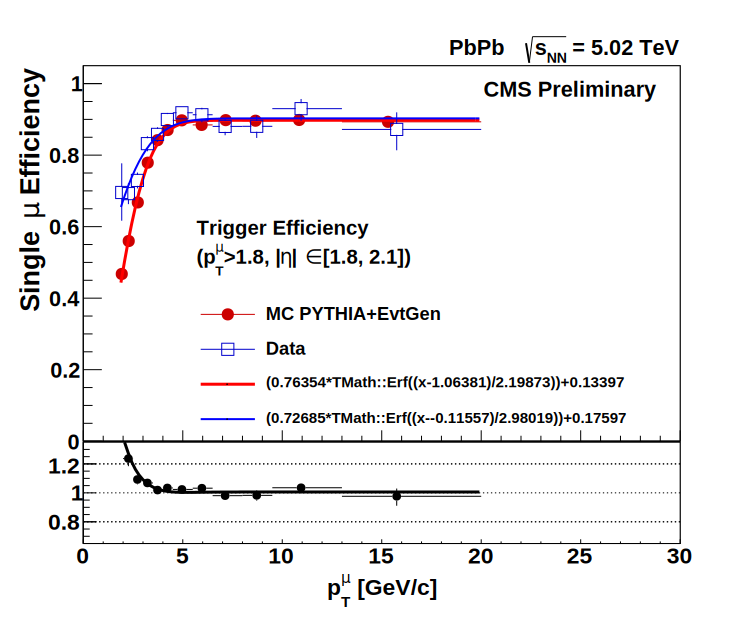
\includegraphics[width=0.45\textwidth]{Figures/Charmonia/Analysis/SignalEfficiency/TnP/tpTreeSF2_PbPb_RD_MC_PT.pdf}
 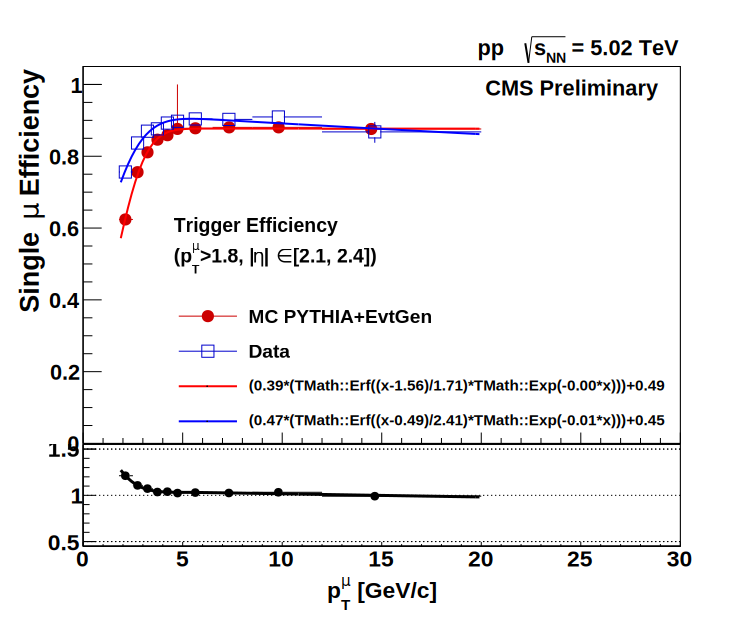
\includegraphics[width=0.45\textwidth]{Figures/Charmonia/Analysis/SignalEfficiency/TnP/tpTreeSF3_pp_RD_MC_PT.pdf}
 \caption{Muon trigger efficiencies as a function of the probe \pt. The efficiencies are extracted, using the \tnp method, from data (blue) and simulation (red) in \RunPbPb collisions at $1.8<|\etaMu|<2.1$ (left) and \Runpp collisions at $2.1<|\etaMu|<2.4$ (right). The bottom panels show the data-to-simulation efficiency ratio. The results of the fits to the efficiencies are also shown. Figures taken from the private Ref.~\cite{Muon_TnP_PbPb}.}
 \label{fig:TnPJpsi}
\end{figure}

The muon trigger efficiencies are measured with respect to the probe \pt, in four $|\eta|$ regions with boundaries: [0.0, 1.2, 1.8, 2.1, 2.4]. The \pt dependence in each $|\eta|$ region is parametrised with a function of the form $f_{\text{trig}}(\pt) = c_{1}\cdot\text{Erf}[(\pt - c_{2})/c_{3}]\cdot\exp[c_{4}\cdot\pt] + c_{5}$, where $\text{Erf}$ is the error function and $c_{i}$ are free parameters. The \tnp-correction weight for the trigger efficiency is then derived from the ratio of the fitted functions, extracted from data and simulation, as a function of probe \pt in each $|\eta|$ region, given by:

\begin{equation}
 w_{\text{trig}}\left(\pt, |\eta|\right) = \left[\frac{f^{\data}_{\text{trig}}\left(\pt\right)}{f^{\MC}_{\text{trig}}\left(\pt\right)}\right]\left({|\eta|}\right)
\end{equation}

To apply the \tnp corrections, the \JPsi-meson efficiency is recomputed by weighing each offline dimuon with the \tnp-correction weights for each muon to trigger, according to:

\begin{equation}
 \effJPsi = \frac{\left[\sum\limits_{i=1}^{N^{\JPsiToMuMu}_{\text{offline}}} w_{\text{trig}}\left(\pt^{\mu,{+}}, |{\eta^{\mu,{+}}}|\right) \cdot w_{\text{trig}}\left(\pt^{\mu,{-}}, |{\eta^{\mu,{-}}}|\right)\right]}{N^{\JPsiToMuMu}_{\gen, \text{\PGm in CMS}}}
\end{equation}

where $\pt^{\mu,{+}(\mu,{-})}$ is the transverse momentum of positive (negative) charged muons, and $\eta^{\mu,{+}(\mu,{-})}$ is the corresponding pseudorapidity. The \tnp corrections increase the \JPsi-meson efficiency by 35\% at $3 < \ptMuMu < 6.5$~\GeVc, while the range of variation at $\ptMuMu > 10$~\GeVc is less than 4\%. The corrected \JPsi-meson efficiencies are shown for \Runpp and \RunPbPb simulated events in \fig{fig:JPsiCorrEff_PP} and  \fig{fig:JPsiCorrEff_PbPb}, respectively.

\begin{figure}[htb!]
 \centering
 \includegraphics[width=0.45\textwidth]{Figures/Charmonia/Analysis/SignalEfficiency/Efficiency/jpsi_pbpb_pt_rap.pdf}
 \includegraphics[width=0.45\textwidth]{Figures/Charmonia/Analysis/SignalEfficiency/Efficiency/npjpsi_pp_rap.pdf}
 \caption{Corrected efficiencies of prompt \JPsi mesons measured in \Runpp collisions, as a function of \ptMuMu (left) and rapidity (right) in different rapidity regions. The error bars represent statistical uncertainties.}
 \label{fig:JPsiCorrEff_PP}
\end{figure}

\begin{figure}[htb!]
 \centering
 \includegraphics[width=0.45\textwidth]{Figures/Charmonia/Analysis/SignalEfficiency/Efficiency/jpsi_pbpb_pt_rap.pdf}
 \includegraphics[width=0.45\textwidth]{Figures/Charmonia/Analysis/SignalEfficiency/Efficiency/jpsi_pbpb_cent_rap.pdf}
 \caption{Corrected efficiencies of prompt \JPsi mesons measured in \RunPbPb collisions, as a function of \ptMuMu (left) and centrality (right), in different rapidity regions. The error bars represent statistical uncertainties.}
 \label{fig:JPsiCorrEff_PbPb}
\end{figure}

\subsubsection{Double ratio of prompt \texorpdfstring{\PsiP}{psi(2S)}/\texorpdfstring{\JPsi}{J/psi} efficiencies}\label{sec:Charmonia_Analysis_Efficiency_Psi2SOverJPsiEfficiency}

Since the prompt \PsiP and \JPsi mesons have similar masses and production mechanisms, it is expected that their efficiencies cancel at first order when measuring the double ratio of prompt charmonium yields in \RunPbPb relative to \Runpp collisions. In order to check this, the efficiency of \PsiP mesons ($\effPsiP$) is estimated from the prompt \PsiPToMuMu simulation, following the same procedure used to determine the \JPsi meson efficiency, described in the previous sections.

The prompt \PsiP and \JPsi meson efficiencies are computed in \Runpp and \RunPbPb collisions, including the \ctau selection defined in \sect{sec:Charmonia_Analysis_PsiPoverJPsiRatioExtraction}, and the double ratio of prompt charmonium efficiencies is then computed as:

\begin{equation}
 \chi^{\PsiP/\JPsi} = \frac{\left(\effPsiP\biggr/\effJPsi\right)_{\PbPb}}{\left(\effPsiP\biggr/\effJPsi\right)_{\pp}}
\end{equation}

The results of the double ratio of prompt charmonium efficiencies are presented in \fig{fig:DoubleRatioEff}. It is observed that the $\chi^{\PsiP/\JPsi}$ is consistent with unity overall as expected. Thus, the measurements of the double ratio of prompt charmonium yields do not require to be  corrected for detector efficiency, and the difference with respect to unity is assigned as a systematic uncertainty as detailed in \sect{sec:Charmonia_Analysis_PsiPoverJPsiRatioSystematics_Effiency}.

\begin{figure}[htb!]
 \centering
 \includegraphics[width=0.45\textwidth]{Figures/Charmonia/Analysis/SignalEfficiency/DoubleRatio/doubleratio_pt_mid_ptdepcut_.pdf}
 \includegraphics[width=0.45\textwidth]{Figures/Charmonia/Analysis/SignalEfficiency/DoubleRatio/doubleratio_pt_fwd_ptdepcut_.pdf}\\
 \includegraphics[width=0.45\textwidth]{Figures/Charmonia/Analysis/SignalEfficiency/DoubleRatio/doubleratio_cent_mid_ptdepcut_.pdf}
 \includegraphics[width=0.45\textwidth]{Figures/Charmonia/Analysis/SignalEfficiency/DoubleRatio/doubleratio_cent_fwd_ptdepcut_.pdf}
 \caption{Double ratios of prompt charmonium efficiencies as a function of \ptMuMu (top) and centrality (bottom), in the rapidity regions: $\abs{\rapMuMu}<1.6$ (left) and $\abs{\rapMuMu}>1.6$ (right). The error bars represent statistical uncertainties.}
 \label{fig:DoubleRatioEff}
\end{figure}


% END OF SUBSECTION

\subsection{Systematic uncertainties of \texorpdfstring{\JPsi}{J/psi}-meson yields}\label{sec:Charmonia_Analysis_JPsiYieldSystematics}

This section describes the procedure used to derive the systematic uncertainties associated to the measurement of the prompt and nonprompt \JPsi-meson yields. The different sources of systematic uncertainties arise from: the parametrisation of the dimuon invariant mass and pseudoproper-decay length  distributions used to extract the signal, and the estimation of the efficiency of \JPsi mesons. In this case, the leading systematic uncertainty of the \JPsi-meson measurements in \Runpp and \RunPbPb collisions correspond to the \tnp efficiency corrections and the \ctau parametrisation, respectively. When describing each systematic source, the corresponding largest relative uncertainty is mentioned.

\subsubsection{Uncertainty on the dimuon invariant mass parametrisation}\label{sec:Charmonia_Analysis_JPsiYieldSystematics_InvMass}

The uncertainty associated to the modelling of the \mMuMu distribution arise from the parametrisation of the signal and background invariant mass shape. It is determined by varying the different components of the \mMuMu functional form and redoing the 2D data fits, while using the nominal \ctau functional form.

\paragraph{Parametrisation of the \texorpdfstring{\JPsi}{J/psi}-meson invariant mass distribution.} In order to estimate the systematic uncertainty associated to the choice of the \JPsi-meson invariant mass shape, two variations are performed:
\begin{itemize}
 \item \textbf{Variation of the \JPsi-meson invariant mass parameters}: the parameters fixed to simulation (i.e. the tail parameters $\aJPsi$ and $\nnJPsi$, and the ratio of CB widths) are released and the data fits are repeated. To improve the convergence of the fits, a set of Gaussian penalty functions, centred in the nominal value of the corresponding parameters, are added to constrain their range of variation.

The range of variation of $\aJPsi$, $\nnJPsi$ and the ratio of CB widths is determined from data by redoing the \mMuMu fits, leaving only one parameter free at the time while the other parameters are fixed to their nominal values. The RMS of the difference between the parameter value extracted from the data fit and the nominal one is computed including the results from different \ptMuMu and centrality intervals within each rapidity region, and the largest RMS obtained among the different rapidity regions is taken as the width of the corresponding Gaussian penalty function. The RMS is defined here as:

\begin{equation}
 \text{RMS} = \sqrt{\frac{1}{\sum_{i}{1/(\sigma_{\text{data}}^{i})^2}} \cdot \sum_{i}{\frac{(\text{par}_{\MC} - \text{par}_{\text{data}}^{i})^2}{(\sigma_{\text{data}}^{i})^2}}}
\end{equation}

where the sum runs over different \pt and centrality bins in the same rapidity region, $\text{par}_{\text{data}}^{i}$ and $\sigma_{\text{data}}^{i}$ is the value and uncertainty of the parameter extracted from the data fit in a given analysis bin $i$, respectively, and $\text{par}_{\MC}$ is the corresponding nominal value derived from simulation. The width of the Gaussian penalty functions of each CB parameter is presented, relative to the nominal parameter value, in \tab{tab:parsRMS}.

\begin{table}[htb!]
  \centering
  \begin{tabular}{lcccc}
    \hline\hline
    System & $\aJPsi$ [\%] & $\nnJPsi$ [\%] & ${\sigma_{\CB,2}/\sigma_{\CB,1}}$ [\%] \\
    \hline
    \Runpp   & 16 & 21 &     \\
    \RunPbPb & 21 & 54 & 30  \\
  \end{tabular}
  \caption{Relative width used in the Gaussian penalty functions for the tail parameters $\aJPsi$ and $n$, and the ratio of CB widths. The Gaussian width is shown relative to the nominal parameter value.}
  \label{tab:parsRMS}
\end{table}

The systematic uncertainty associated to the determination of the signal mass parameters from simulations is then estimated by performing the data fits with the Gaussian penalty functions, and the difference between the varied \JPsi-meson yields and the nominal results is taken as the uncertainty.

 \item \textbf{Variation of the \JPsi-meson invariant mass model}: the functional form of the signal invariant mass shape is changed from the nominal double Crystal Ball function to a Crystal Ball plus a Gaussian function (with common mean parameters), defined as:

\begin{equation}
  M_{\JPsi}\left(m_{\mumu}\right) = \fJPsi \cdot \CB\left(\mMuMu\right) + \left(1- \fJPsi\right) \cdot \Gauss\left(\mMuMu\right)
\end{equation}

As in the nominal case, the parameters of the alternative signal \mMuMu model are tuned from fits to the \JPsi-meson simulations, and the tail parameters \aJPsi and \nnJPsi are fixed to simulation in both \Runpp and \RunPbPb data fits, while the ratio of CB over Gaussian widths ($\sigma_{\CB}/\sigma_{\text{G}}$) is fixed only in the \RunPbPb data fits.

\end{itemize}

The systematic uncertainty on the signal shape parametrisation is then determined from the quadratic sum of the uncertainties obtained from varying the invariant mass parameters and the shape model. The corresponding uncertainty for prompt and nonprompt \JPsi mesons amounts to 1.2\% (2.7\%) and 2.4\% (2.7\%), in \Runpp (\RunPbPb) collisions, respectively.

\paragraph{Parametrisation of the background invariant mass shape.} In the case of the background invariant mass parametrisation, three variations are performed to derive the corresponding systematic uncertainty, given by:

\begin{itemize}
 \item \textbf{Variation of the LLR test threshold}: the $\chi^{2}$ probability threshold is increased from the nominal value (5\%) to 10\% and reduced to 2.5\%, and the LLR tests are repeated for each threshold. The background models selected from each LLR test are then used to redo the 2D fits.
 
 \item \textbf{Variation of the dimuon invariant mass fitting range}: the range of the \mMuMu distribution used in the 2D fits is changed from 2.6-3.5~\GeVcc to 2.6-3.4~\GeVcc. The 2D fits are then remade using the same orders of Chebyshev functions as used in the nominal fits.
 
 \item \textbf{Variation of the background invariant mass model}: the background \mMuMu functional form is changed from the nominal Chebyshev function to an exponential of a Chebyshev function, defined as:

\begin{equation}
 M_{\bkg}^{N}\left(\mMuMu\right) = \exp\left[\sum_{i=0}^{N} {c_{i} T_{i}\left(\mMuMu\right)}\right]
\end{equation}

where $T$ are Chebyshev polynomials and $c$ are free parameters. As in the nominal analysis, the \mMuMu distribution in data is fitted using the alternative background model with orders between 0 and 6, and the LLR test is employed with a 5\% threshold to decide the best order in each analysis bin.
  
\end{itemize}

The uncertainty associated to each systematic variation is determined by computing the deviation of the measured prompt and nonprompt \JPsi-meson yields from the nominal results. In the case of the two variations done for the LLR test threshold, the maximum deviation between the two variations is taken for each \JPsi-meson yield. The systematic uncertainties of the different sources are combined by adding them in quadrature. The combined uncertainty amounts to 0.6\% (3.0\%) for prompt \JPsi mesons and 1.6\% (2.9\%) for nonprompt \JPsi mesons, in \Runpp (\RunPbPb) collisions.


\subsubsection{Uncertainty on the pseudoproper-decay length parametrisation}\label{sec:Charmonia_Analysis_JPsiYieldSystematics_Ctau}

The different systematic variations performed for the pseudoproper-decay length parametrisation are summarised as follows:

\begin{enumerate}
 \item Modelling of the \sigmactau distribution: replace the nominal signal and background \sigmactau templates in the 2D fits with the template of the total \sigmactau distribution.
 \item Parametrisation of the \ctau resolution: parametrise the \ctau resolution model using the simulated sample of prompt \JPsi mesons instead of data.
 \item Parametrisation of the nonprompt \JPsi-meson \ctau shape: replace the exponential \ctau model used to describe nonprompt \JPsi mesons in the 2D fits with a template of the \ctau distribution derived from simulation.
 \item Parametrisation of the background \ctau shape: use a template of the \ctau distribution from the background-like dataset derived with \sPlot, instead of a functional form.
\end{enumerate}

The method and result of these four sources are detailed below, and the resulting uncertainties are summed in quadrature with the other systematic sources.

\paragraph{Modelling of the \sigmactau distribution.} To estimate the uncertainty associated to the use of the signal and background \sigmactau template histograms, derived from the \sPlot background- and signal-like datasets, the template histograms of the signal and background are made instead using the full \sigmactau distribution and the 2D fits are remade. The difference between the varied and nominal \JPsi meson yields is taken as the systematic uncertainty, which amounts to 0.6\% (6.3\%) for prompt \JPsi mesons and 2.1\% (4.2\%) for nonprompt \JPsi mesons, in \Runpp (\RunPbPb) collisions.

\paragraph{Parametrisation of the \ctau resolution.} The systematic uncertainty due to the parametrisation of the \ctau resolution is estimated by extracting the \ctau resolution parameters from \JPsi-meson simulations instead of the data. The \ctau resolution parameters are extracted from simulated samples of prompt \JPsi mesons by fitting the nominal \ctau resolution model (weighed sum of three Gaussians) to the simulated \ctau distribution. The varied \ctau resolution parameters are then used to remake the 2D fits and the uncertainty is derived from the difference between the varied \JPsi-meson yields and the nominal ones. This systematic uncertainty amounts in \Runpp (\RunPbPb) collisions to 1.5\% (4.7\%) for prompt \JPsi mesons and 5.3\% (9.6\%) for nonprompt \JPsi mesons.

\paragraph{Parametrisation of the nonprompt \JPsi-meson \ctau shape.} The systematic uncertainty associated to the modelling of the \ctau distribution of nonprompt \JPsi mesons is computed by replacing the nominal signal functional form (convolution of exponential decay with \ctau resolution model) with an unbinned template of the reconstructed \ctau distribution derived from simulation of nonprompt \JPsi mesons. The \ctau templates are made using a kernel estimation technique~\cite{RooKeysPDF}, implemented in the RooFit framework, which parametrise the distribution of a given variable by superimposing a Gaussian function to each data point. The uncertainty is then determined from the difference between the varied signal yields and the nominal results, and reaches up to 0.8\% (3.4\%) for prompt \JPsi mesons and 2.1\% (12.1\%) for nonprompt \JPsi mesons, in \Runpp (\RunPbPb) collisions.

\paragraph{Parametrisation of the background \ctau shape.} The systematic uncertainty related to the choice of background \ctau model is determined by replacing the nominal background functional form (three exponential decay functions convolved with the \ctau resolution model) with an unbinned template. The template is built from the \ctau distribution of the \sPlot background-like dataset employed in \sect{sec:Charmonia_Analysis_JPsiYieldExtraction_CtauPar}, using the RooFit kernel estimation technique. This uncertainty contributes in \Runpp (\RunPbPb) collisions up to 0.5\% (10\%) for prompt \JPsi mesons and 1.2\% (22.3\%) for nonprompt \JPsi mesons.


\subsubsection{Uncertainty on the \texorpdfstring{\JPsi}{J/psi}-meson efficiency}\label{sec:Charmonia_Analysis_JPsiYieldSystematics_Efficiency}

There are two main sources of systematics that affects the measurement of the \JPsi-meson efficiencies: the \tnp-correction weights used to correct the simulated efficiencies and the charmonium $\ptMuMu$-$\rapMuMu$ weights applied to improve the modelling of the \JPsi-meson \pt and rapidity. Among these two, the largest uncertainty is obtained from the \tnp corrections, which is dominated by the uncertainty on the extraction of the standalone-muon reconstruction efficiency in data.

\paragraph{Tag-and-probe correction.} The uncertainty associated to the \tnp correction derives from the measurement of the \tnp data efficiency of muon identification, trigger, tracking and standalone-muon reconstruction.

Regarding the tracking efficiency, an overall systematic uncertainty is determined from the largest difference found between data and simulation, which corresponds to a relative uncertainty on the \JPsi-meson yields measured in \Runpp and \RunPbPb collisions of 1.0\% and 2.4\%, respectively. On the other hand, for the standalone-muon reconstruction, trigger and muon identification, the uncertainties of the \tnp-correction weights are separated in a statistical and systematic component. The statistical component of the \tnp-correction uncertainty is evaluated by producing a hundred sets of \tnp-correction weights, where each point is randomly generated using a Gaussian distribution spread according to its statistical uncertainty. The hundred sets of \tnp-correction weights are then used to recompute the \JPsi-meson efficiencies and the corresponding systematic uncertainty is estimated by computing the RMS of the hundred variations of the prompt and nonprompt \JPsi-meson efficiencies. The systematic component of the \tnp-correction uncertainty is propagated using two sets of \tnp-correction weights generated by shifting all points up and down, according to the systematic uncertainty of each point (derived by varying the settings of the \tnp invariant mass fits). The \JPsi-meson efficiencies are then corrected with each set of \tnp-correction  weights and the maximum deviation of the two varied efficiencies with respect to the nominal one is taken as the systematic uncertainty on the efficiency of prompt and nonprompt \JPsi mesons.

The statistical component of the \tnp uncertainty represents 1.5\% (4.6\%) for the \Runpp (\RunPbPb) efficiencies. Regarding the systematic components of the \tnp uncertainty, the largest uncertainty is obtained from the standalone-muon reconstruction efficiency, which corresponds to 9.6\%, while the \tnp-correction uncertainties associated to the trigger and muon identification efficiencies in \Runpp (\RunPbPb) collisions amounts to 0.5\% (5.2\%) and to 1.1\% (3.3\%), respectively.

\paragraph{Charmonium transverse momentum and rapidity weighing.} The simulated samples of \JPsi mesons are weighed as a function of dimuon \pt and rapidity, to match the \pt spectrum of prompt and nonprompt \JPsi mesons observed in data in four rapidity regions. In order to estimate the uncertainty of the weighing procedure, a hundred sets of weights are randomly generated using a Gaussian distribution for each $\ptMuMu$-$\rapMuMu$ interval, where the Gaussian width is fixed to the uncertainty of the corresponding dimuon kinematic weight. The simulations are reweighed with each set of generated dimuon kinematic weights and then used to recompute the efficiencies of prompt and nonprompt \JPsi mesons. The corresponding systematic uncertainty is then determined from the RMS of the hundred varied efficiencies compared to the nominal efficiency for prompt and nonprompt \JPsi mesons. In this case, the largest relative uncertainty on the \Runpp (\RunPbPb) \JPsi-meson efficiencies corresponds to 0.2\% (1.8\%).


% END OF SUBSECTION

\subsection{Systematic uncertainties on the \texorpdfstring{\PsiP}{psi(2S)}/\texorpdfstring{\JPsi}{J/psi} ratio}\label{sec:Charmonia_Analysis_PsiPoverJPsiRatioSystematics}

This section is dedicated to the systematic uncertainties that contributes in the measurement of the \doubleRatio double ratio. Three sources of systematics are accounted for: the parametrisation of the dimuon invariant mass used in the signal extraction, the degree of cancellation of the charmonium efficiencies in the double ratio and the subtraction of the nonprompt charmonium component.

\subsubsection{Uncertainty on the dimuon invariant mass parametrisation}\label{sec:Charmonia_Analysis_PsiPoverJPsiRatioSystematics_InvMass}

A large part of the method used to determine the uncertainty on the signal and background \mMuMu shape  parametrisation is common to the one used for the prompt and nonprompt \JPsi meson yields, presented in \sect{sec:Charmonia_Analysis_JPsiYieldSystematics_InvMass}. Indeed, the \PsiP-to-\JPsi double ratio analysis was performed first and was less demanding in terms of systematic uncertainties, due to the limited \PsiP statistics. However, it served as a basis for the \JPsi-meson yield analysis and all the sources considered here were kept.

The functional forms of the \JPsi-meson, \PsiP-meson and background invariant mass shape are varied accordingly and the fits to data are remade. The nominal background shape is used when varying the signal functional form and vice versa. The variations performed on the signal functional forms includes:
\begin{itemize}
 \item varying the CB parameters fixed to simulation ($\aJPsi$, $\nnJPsi$ and $\sigma_{\CB,2}/\sigma_{\CB,1}$) in the following way:
  \begin{enumerate}
   \item setting $\aJPsi$ free while keeping $\nnJPsi$ (and $\sigma_{\CB,2}/\sigma_{\CB,1}$ in \RunPbPb fits) fixed to simulation;
   \item setting $\nnJPsi$ free while keeping $\aJPsi$ fixed (only done for \Runpp data since the \RunPbPb data fits did not converge);
   \item fixing the CB parameters to their corresponding values derived from the prompt \PsiP-meson simulation, instead of the \JPsi-meson simulation.
  \end{enumerate}
  \item changing the signal shape model by using a Gaussian plus a Crystal Ball function (with common mean), instead of the nominal double Crystal Ball function. The alternative model parameters are tuned and fixed in the same way as done for the nominal model;
\end{itemize}

In the case of the background functional form, the following variations are done:
\begin{itemize}
 \item the fitted dimuon invariant mass range is changed to 2.2-4.2~\GeVcc, instead of 2.2-4.5~\GeVcc;
 \item the background shape model is changed to an exponential of a Chebyshev function, instead of the nominal Chebyshev function. The LLR tests are remade to determine the best order of the exponent in each analysis bin;
 \item the LLR test selection criteria is changed by varying the $\chi^{2}$-probability threshold to 10\% and 2.5\%, instead of nominal 5\%.
\end{itemize}

For each source of uncertainty (choice of signal and background models), the maximum difference between the \singleRatio ratio extracted from the varied data fits and the nominal results defines the uncertainty on the single ratio of charmonium yields. This procedure is performed separately for \Runpp and \RunPbPb collisions, and the corresponding uncertainties on the single ratios are then propagated to the double ratio.

The largest relative uncertainty on the \singleRatio ratio from the signal parametrisation derives from changing the signal shape model and corresponds to 1.9\% (18.5\%) in \Runpp (\RunPbPb) collisions. In the case of the background parametrisation, the largest relative uncertainty arises from the LLR test (5.3\%) in \Runpp data and from changing the background shape model (37.3\%) in \RunPbPb data.


\subsubsection{Uncertainty on the cancellation of the double ratio of efficiencies}\label{sec:Charmonia_Analysis_PsiPoverJPsiRatioSystematics_Effiency}

The cancellation of the double ratio of \PsiP over \JPsi meson efficiencies is verified up to a finite degree of precision determined by the statistical precision of the simulations and the modelling of the charmonium kinematic spectra. In this case, the following sources of systematic uncertainties are taken into account: 
\begin{itemize}
 \item the statistical uncertainty of the double ratio of efficiencies extracted from the simulated samples (i.e. the error bars in \fig{fig:DoubleRatioEff});
 \item the difference between unity and the value of the double ratio of efficiencies computed after weighing per-event the simulated dimuon \pt spectrum to the corresponding charmonium \pt distribution observed in data (the charmonium \pt spectrum in data is extracted from the nominal fits);
 \item the spread of the double ratio of efficiencies determined with MC studies, considering the range of \pt spectra compatible with the \RunPbPb and \Runpp data. This is done by generating a hundred random \pt distributions of the charmonium \pt spectrum extracted from the nominal data fits, where each data point is randomised following a Gaussian distribution with mean and width equal to the nominal value and statistical uncertainty, respectively. Then the simulated dimuon \pt spectrum is weighed, event-by-event, to match each of the generated random \pt distributions, and in each case, the double ratio of efficiencies is computed. The RMS of the one hundred efficiency double ratio values is taken as the systematic uncertainty.
\end{itemize}

These three sources of uncertainties are summed in quadrature. In this case, the largest relative uncertainty on the double ratio of charmonium yields amounts to 20\%.

\subsubsection{Uncertainty on the substraction of nonprompt charmonia}\label{sec:Charmonia_Analysis_PsiPoverJPsiRatioSystematics_NPCorr}

The nominal method used to subtract the nonprompt charmonium contamination relies on simulations to determine the expected fraction of prompt and nonprompt charmonia passing and failing the \ctau selection. To determine the uncertainty on this procedure, a set of 2D fits are employed using the same procedure employed in Ref.~\cite{CMS_JPsi_PbPb_2p76TeV}, which is similar to the one presented in this chapter.

The 2D fits are performed in two dimuon invariant mass ranges: 2.2-3.5~\GeVcc and 3.3-4.4~\GeVcc. The first one is used to extract the fraction of nonprompt \JPsi mesons in \Runpp and \RunPbPb data, while the second range is used to derive the nonprompt \PsiP meson fraction from \Runpp data only. The prompt charmonium yields are then computed using the nonprompt charmonium fractions extracted from the 2D fits ($f^{\text{NP}, \text{2D}}_{\psi}$), as given by:

\begin{equation}
 N^{\text{P}, \text{2D}}_{\psi} = \left(1 - f^{\text{NP}, \text{2D}}_{\psi}\right)N^{\text{tot}}_{\psi}
 \label{eq:2DPsi2SSyst}
\end{equation}

where $N^{\text{tot}}_{\psi}$ is the total number of charmonia extracted from the nominal fits.

In the case of \PsiP mesons in \RunPbPb collisions, the number of prompt \PsiP mesons is derived according to:

\begin{equation}
 N^{\text{P}, \text{2D}}_{\PsiP, \PbPb} =  N^{\text{P}, \text{nominal}}_{\PsiP, \PbPb}\times\left(\frac{N^{\text{P}, \text{2D}}_{\PsiP, \pp}}{N^{\text{P}, \text{nominal}}_{\PsiP, \pp}}\right)
 \label{eq:2DPsi2SSyst_2}
\end{equation}

where $N^{\text{P}, \text{nominal}}_{\PsiP}$ is the number of prompt \PsiP mesons determined in the  nominal case, as presented in \sect{sec:Charmonia_Analysis_PsiPYieldExtraction_NonPromptCorr}. 

The double ratio is then recomputed using the prompt charmonium yields derived from \eq{eq:2DPsi2SSyst} and \eq{eq:2DPsi2SSyst_2}. The difference between the double ratio of charmonium yields when accounting for the nonprompt charmonium contamination using the nominal method and using 2D fits, is taken as a systematic uncertainty. The largest relative uncertainty is found to be 17.7\%.


% END OF SUBSECTION
